\documentclass[12pt]{article}
\usepackage[letterpaper,top=0.8in,bottom=0.8in,left=0.5in,right=0.5in,
            headheight=15pt,headsep=0.25in,footskip=0.4in]{geometry}
\usepackage[T1]{fontenc}
\usepackage{helvet}
\renewcommand{\familydefault}{\sfdefault}
\usepackage{tikz}
\usetikzlibrary{shapes.geometric}
\usepackage{fancyhdr}
\usepackage{xcolor}

\definecolor{redtint}{RGB}{248,180,172}
\definecolor{bluetint}{RGB}{110,150,215}
\definecolor{redctr}{RGB}{235,95,85}
\definecolor{bluectr}{RGB}{30,70,160}
\definecolor{gridline}{RGB}{60,60,60}
\definecolor{writeline}{RGB}{185,185,185}

\pagestyle{fancy}
\fancyhf{}
\lhead{Week NN / Hex / Grades 4--5}
\lfoot{Bellingham Math Circle / Week NN / HEX-45-v1}
\rfoot{\thepage}
\renewcommand{\headrulewidth}{0pt}
\setlength{\parindent}{0pt}
\setlength{\parskip}{0pt}
\newcommand{\prob}[1]{\textbf{Problem #1:}}
\newsavebox{\landbox}
\begin{document}
\large\raggedright
\begin{minipage}[c]{0.56\textwidth}\raggedright Red and Blue take turns putting a counter of their own color on an empty hexagon. Red wins by joining the two red edges with a chain of red hexagons. Blue wins by joining the two blue edges with a chain of blue hexagons. Each hexagon in a chain shares a side with the next one.\end{minipage}\hfill\begin{minipage}[c]{0.38\textwidth}\centering 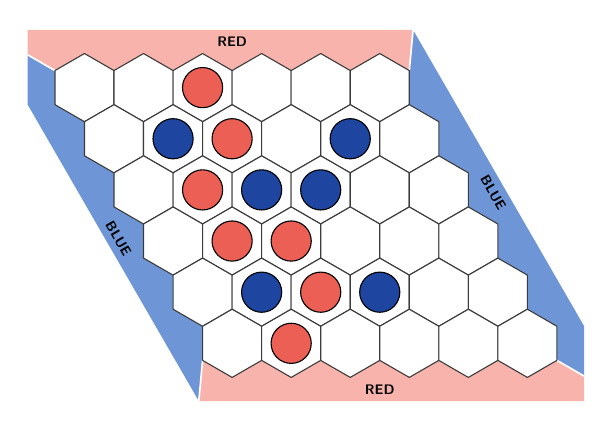
\begin{tikzpicture}[x=1.0mm,y=1.0mm,line join=round]
\begin{scope}
\clip (-7.214,-39.806) rectangle (63.464,7.330);
\fill[redtint] (-3.750,2.165) -- (0.000,4.330) -- (3.750,2.165) -- (7.500,4.330) -- (11.250,2.165) -- (15.000,4.330) -- (18.750,2.165) -- (22.500,4.330) -- (26.250,2.165) -- (30.000,4.330) -- (33.750,2.165) -- (37.500,4.330) -- (41.250,2.165) -- (41.732,7.330) -- (-12.696,7.330) -- cycle;
\fill[redtint] (60.000,-34.641) -- (56.250,-36.806) -- (52.500,-34.641) -- (48.750,-36.806) -- (45.000,-34.641) -- (41.250,-36.806) -- (37.500,-34.641) -- (33.750,-36.806) -- (30.000,-34.641) -- (26.250,-36.806) -- (22.500,-34.641) -- (18.750,-36.806) -- (15.000,-34.641) -- (14.518,-39.806) -- (68.946,-39.806) -- cycle;
\fill[bluetint] (15.000,-34.641) -- (15.000,-30.311) -- (11.250,-28.146) -- (11.250,-23.816) -- (7.500,-21.651) -- (7.500,-17.321) -- (3.750,-15.155) -- (3.750,-10.825) -- (0.000,-8.660) -- (-0.000,-4.330) -- (-3.750,-2.165) -- (-3.750,2.165) -- (-12.696,7.330) -- (14.518,-39.806) -- cycle;
\fill[bluetint] (41.250,2.165) -- (41.250,-2.165) -- (45.000,-4.330) -- (45.000,-8.660) -- (48.750,-10.825) -- (48.750,-15.155) -- (52.500,-17.321) -- (52.500,-21.651) -- (56.250,-23.816) -- (56.250,-28.146) -- (60.000,-30.311) -- (60.000,-34.641) -- (68.946,-39.806) -- (41.732,7.330) -- cycle;
\draw[white,line width=0.6pt] (-3.750,2.165) -- (-12.696,7.330);
\draw[white,line width=0.6pt] (41.250,2.165) -- (41.732,7.330);
\draw[white,line width=0.6pt] (60.000,-34.641) -- (68.946,-39.806);
\draw[white,line width=0.6pt] (15.000,-34.641) -- (14.518,-39.806);
\end{scope}
\node[font=\tiny\bfseries,text=black] at (18.750,5.830) {RED};
\node[font=\tiny\bfseries,text=black] at (37.500,-38.306) {RED};
\node[font=\tiny\bfseries,text=black,rotate=-60] at (4.326,-19.153) {BLUE};
\node[font=\tiny\bfseries,text=black,rotate=-60] at (51.924,-13.323) {BLUE};
\filldraw[fill=white,draw=gridline,line width=0.4pt] (3.750,2.165) -- (0.000,4.330) -- (-3.750,2.165) -- (-3.750,-2.165) -- (-0.000,-4.330) -- (3.750,-2.165) -- cycle;
\filldraw[fill=white,draw=gridline,line width=0.4pt] (11.250,2.165) -- (7.500,4.330) -- (3.750,2.165) -- (3.750,-2.165) -- (7.500,-4.330) -- (11.250,-2.165) -- cycle;
\filldraw[fill=white,draw=gridline,line width=0.4pt] (18.750,2.165) -- (15.000,4.330) -- (11.250,2.165) -- (11.250,-2.165) -- (15.000,-4.330) -- (18.750,-2.165) -- cycle;
\filldraw[fill=white,draw=gridline,line width=0.4pt] (26.250,2.165) -- (22.500,4.330) -- (18.750,2.165) -- (18.750,-2.165) -- (22.500,-4.330) -- (26.250,-2.165) -- cycle;
\filldraw[fill=white,draw=gridline,line width=0.4pt] (33.750,2.165) -- (30.000,4.330) -- (26.250,2.165) -- (26.250,-2.165) -- (30.000,-4.330) -- (33.750,-2.165) -- cycle;
\filldraw[fill=white,draw=gridline,line width=0.4pt] (41.250,2.165) -- (37.500,4.330) -- (33.750,2.165) -- (33.750,-2.165) -- (37.500,-4.330) -- (41.250,-2.165) -- cycle;
\filldraw[fill=white,draw=gridline,line width=0.4pt] (7.500,-4.330) -- (3.750,-2.165) -- (-0.000,-4.330) -- (0.000,-8.660) -- (3.750,-10.825) -- (7.500,-8.660) -- cycle;
\filldraw[fill=white,draw=gridline,line width=0.4pt] (15.000,-4.330) -- (11.250,-2.165) -- (7.500,-4.330) -- (7.500,-8.660) -- (11.250,-10.825) -- (15.000,-8.660) -- cycle;
\filldraw[fill=white,draw=gridline,line width=0.4pt] (22.500,-4.330) -- (18.750,-2.165) -- (15.000,-4.330) -- (15.000,-8.660) -- (18.750,-10.825) -- (22.500,-8.660) -- cycle;
\filldraw[fill=white,draw=gridline,line width=0.4pt] (30.000,-4.330) -- (26.250,-2.165) -- (22.500,-4.330) -- (22.500,-8.660) -- (26.250,-10.825) -- (30.000,-8.660) -- cycle;
\filldraw[fill=white,draw=gridline,line width=0.4pt] (37.500,-4.330) -- (33.750,-2.165) -- (30.000,-4.330) -- (30.000,-8.660) -- (33.750,-10.825) -- (37.500,-8.660) -- cycle;
\filldraw[fill=white,draw=gridline,line width=0.4pt] (45.000,-4.330) -- (41.250,-2.165) -- (37.500,-4.330) -- (37.500,-8.660) -- (41.250,-10.825) -- (45.000,-8.660) -- cycle;
\filldraw[fill=white,draw=gridline,line width=0.4pt] (11.250,-10.825) -- (7.500,-8.660) -- (3.750,-10.825) -- (3.750,-15.155) -- (7.500,-17.321) -- (11.250,-15.155) -- cycle;
\filldraw[fill=white,draw=gridline,line width=0.4pt] (18.750,-10.825) -- (15.000,-8.660) -- (11.250,-10.825) -- (11.250,-15.155) -- (15.000,-17.321) -- (18.750,-15.155) -- cycle;
\filldraw[fill=white,draw=gridline,line width=0.4pt] (26.250,-10.825) -- (22.500,-8.660) -- (18.750,-10.825) -- (18.750,-15.155) -- (22.500,-17.321) -- (26.250,-15.155) -- cycle;
\filldraw[fill=white,draw=gridline,line width=0.4pt] (33.750,-10.825) -- (30.000,-8.660) -- (26.250,-10.825) -- (26.250,-15.155) -- (30.000,-17.321) -- (33.750,-15.155) -- cycle;
\filldraw[fill=white,draw=gridline,line width=0.4pt] (41.250,-10.825) -- (37.500,-8.660) -- (33.750,-10.825) -- (33.750,-15.155) -- (37.500,-17.321) -- (41.250,-15.155) -- cycle;
\filldraw[fill=white,draw=gridline,line width=0.4pt] (48.750,-10.825) -- (45.000,-8.660) -- (41.250,-10.825) -- (41.250,-15.155) -- (45.000,-17.321) -- (48.750,-15.155) -- cycle;
\filldraw[fill=white,draw=gridline,line width=0.4pt] (15.000,-17.321) -- (11.250,-15.155) -- (7.500,-17.321) -- (7.500,-21.651) -- (11.250,-23.816) -- (15.000,-21.651) -- cycle;
\filldraw[fill=white,draw=gridline,line width=0.4pt] (22.500,-17.321) -- (18.750,-15.155) -- (15.000,-17.321) -- (15.000,-21.651) -- (18.750,-23.816) -- (22.500,-21.651) -- cycle;
\filldraw[fill=white,draw=gridline,line width=0.4pt] (30.000,-17.321) -- (26.250,-15.155) -- (22.500,-17.321) -- (22.500,-21.651) -- (26.250,-23.816) -- (30.000,-21.651) -- cycle;
\filldraw[fill=white,draw=gridline,line width=0.4pt] (37.500,-17.321) -- (33.750,-15.155) -- (30.000,-17.321) -- (30.000,-21.651) -- (33.750,-23.816) -- (37.500,-21.651) -- cycle;
\filldraw[fill=white,draw=gridline,line width=0.4pt] (45.000,-17.321) -- (41.250,-15.155) -- (37.500,-17.321) -- (37.500,-21.651) -- (41.250,-23.816) -- (45.000,-21.651) -- cycle;
\filldraw[fill=white,draw=gridline,line width=0.4pt] (52.500,-17.321) -- (48.750,-15.155) -- (45.000,-17.321) -- (45.000,-21.651) -- (48.750,-23.816) -- (52.500,-21.651) -- cycle;
\filldraw[fill=white,draw=gridline,line width=0.4pt] (18.750,-23.816) -- (15.000,-21.651) -- (11.250,-23.816) -- (11.250,-28.146) -- (15.000,-30.311) -- (18.750,-28.146) -- cycle;
\filldraw[fill=white,draw=gridline,line width=0.4pt] (26.250,-23.816) -- (22.500,-21.651) -- (18.750,-23.816) -- (18.750,-28.146) -- (22.500,-30.311) -- (26.250,-28.146) -- cycle;
\filldraw[fill=white,draw=gridline,line width=0.4pt] (33.750,-23.816) -- (30.000,-21.651) -- (26.250,-23.816) -- (26.250,-28.146) -- (30.000,-30.311) -- (33.750,-28.146) -- cycle;
\filldraw[fill=white,draw=gridline,line width=0.4pt] (41.250,-23.816) -- (37.500,-21.651) -- (33.750,-23.816) -- (33.750,-28.146) -- (37.500,-30.311) -- (41.250,-28.146) -- cycle;
\filldraw[fill=white,draw=gridline,line width=0.4pt] (48.750,-23.816) -- (45.000,-21.651) -- (41.250,-23.816) -- (41.250,-28.146) -- (45.000,-30.311) -- (48.750,-28.146) -- cycle;
\filldraw[fill=white,draw=gridline,line width=0.4pt] (56.250,-23.816) -- (52.500,-21.651) -- (48.750,-23.816) -- (48.750,-28.146) -- (52.500,-30.311) -- (56.250,-28.146) -- cycle;
\filldraw[fill=white,draw=gridline,line width=0.4pt] (22.500,-30.311) -- (18.750,-28.146) -- (15.000,-30.311) -- (15.000,-34.641) -- (18.750,-36.806) -- (22.500,-34.641) -- cycle;
\filldraw[fill=white,draw=gridline,line width=0.4pt] (30.000,-30.311) -- (26.250,-28.146) -- (22.500,-30.311) -- (22.500,-34.641) -- (26.250,-36.806) -- (30.000,-34.641) -- cycle;
\filldraw[fill=white,draw=gridline,line width=0.4pt] (37.500,-30.311) -- (33.750,-28.146) -- (30.000,-30.311) -- (30.000,-34.641) -- (33.750,-36.806) -- (37.500,-34.641) -- cycle;
\filldraw[fill=white,draw=gridline,line width=0.4pt] (45.000,-30.311) -- (41.250,-28.146) -- (37.500,-30.311) -- (37.500,-34.641) -- (41.250,-36.806) -- (45.000,-34.641) -- cycle;
\filldraw[fill=white,draw=gridline,line width=0.4pt] (52.500,-30.311) -- (48.750,-28.146) -- (45.000,-30.311) -- (45.000,-34.641) -- (48.750,-36.806) -- (52.500,-34.641) -- cycle;
\filldraw[fill=white,draw=gridline,line width=0.4pt] (60.000,-30.311) -- (56.250,-28.146) -- (52.500,-30.311) -- (52.500,-34.641) -- (56.250,-36.806) -- (60.000,-34.641) -- cycle;
\filldraw[fill=redctr,draw=black,line width=0.4pt] (15.000,0.000) circle (2.550);
\filldraw[fill=redctr,draw=black,line width=0.4pt] (18.750,-6.495) circle (2.550);
\filldraw[fill=redctr,draw=black,line width=0.4pt] (15.000,-12.990) circle (2.550);
\filldraw[fill=redctr,draw=black,line width=0.4pt] (18.750,-19.486) circle (2.550);
\filldraw[fill=redctr,draw=black,line width=0.4pt] (26.250,-19.486) circle (2.550);
\filldraw[fill=redctr,draw=black,line width=0.4pt] (30.000,-25.981) circle (2.550);
\filldraw[fill=redctr,draw=black,line width=0.4pt] (26.250,-32.476) circle (2.550);
\filldraw[fill=bluectr,draw=black,line width=0.4pt] (11.250,-6.495) circle (2.550);
\filldraw[fill=bluectr,draw=black,line width=0.4pt] (22.500,-12.990) circle (2.550);
\filldraw[fill=bluectr,draw=black,line width=0.4pt] (30.000,-12.990) circle (2.550);
\filldraw[fill=bluectr,draw=black,line width=0.4pt] (22.500,-25.981) circle (2.550);
\filldraw[fill=bluectr,draw=black,line width=0.4pt] (37.500,-25.981) circle (2.550);
\filldraw[fill=bluectr,draw=black,line width=0.4pt] (33.750,-6.495) circle (2.550);
\end{tikzpicture}\end{minipage}
\par\vspace{7mm}
\prob{1} Play Hex on this board. Take turns going first.
\begin{center}
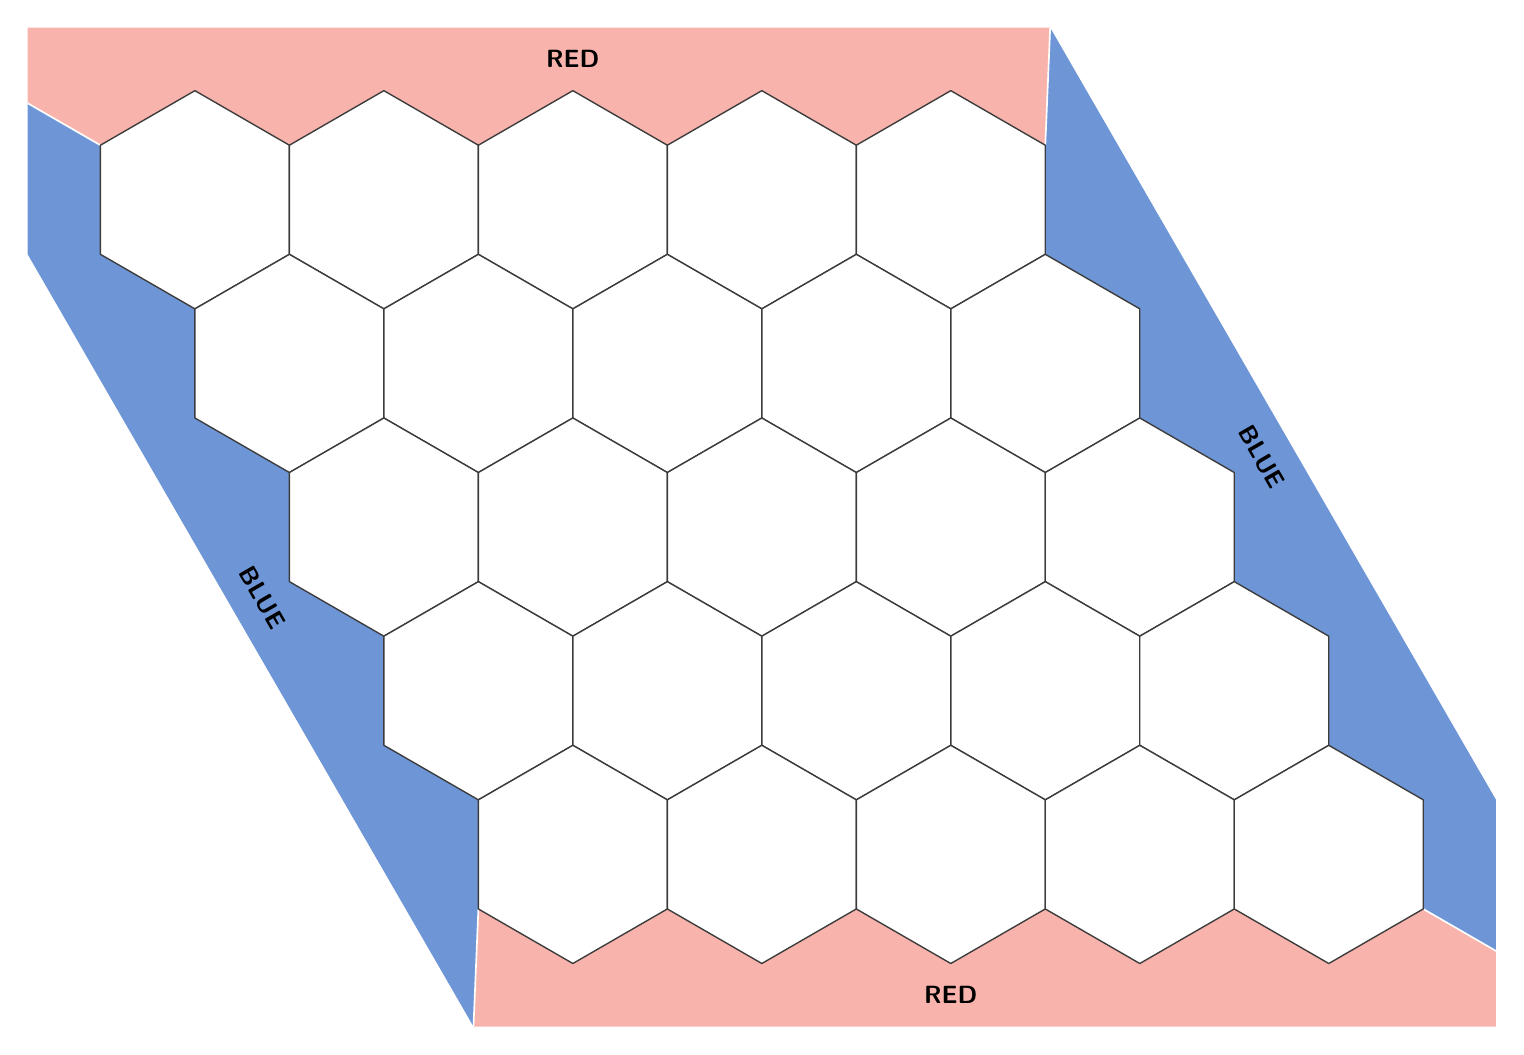
\begin{tikzpicture}[x=1.0mm,y=1.0mm,line join=round]
\begin{scope}
\clip (-21.238,-104.995) rectangle (165.238,21.856);
\fill[redtint] (-12.000,6.928) -- (0.000,13.856) -- (12.000,6.928) -- (24.000,13.856) -- (36.000,6.928) -- (48.000,13.856) -- (60.000,6.928) -- (72.000,13.856) -- (84.000,6.928) -- (96.000,13.856) -- (108.000,6.928) -- (108.619,21.856) -- (-37.856,21.856) -- cycle;
\fill[redtint] (156.000,-90.067) -- (144.000,-96.995) -- (132.000,-90.067) -- (120.000,-96.995) -- (108.000,-90.067) -- (96.000,-96.995) -- (84.000,-90.067) -- (72.000,-96.995) -- (60.000,-90.067) -- (48.000,-96.995) -- (36.000,-90.067) -- (35.381,-104.995) -- (181.856,-104.995) -- cycle;
\fill[bluetint] (36.000,-90.067) -- (36.000,-76.210) -- (24.000,-69.282) -- (24.000,-55.426) -- (12.000,-48.497) -- (12.000,-34.641) -- (0.000,-27.713) -- (-0.000,-13.856) -- (-12.000,-6.928) -- (-12.000,6.928) -- (-37.856,21.856) -- (35.381,-104.995) -- cycle;
\fill[bluetint] (108.000,6.928) -- (108.000,-6.928) -- (120.000,-13.856) -- (120.000,-27.713) -- (132.000,-34.641) -- (132.000,-48.497) -- (144.000,-55.426) -- (144.000,-69.282) -- (156.000,-76.210) -- (156.000,-90.067) -- (181.856,-104.995) -- (108.619,21.856) -- cycle;
\draw[white,line width=0.6pt] (-12.000,6.928) -- (-37.856,21.856);
\draw[white,line width=0.6pt] (108.000,6.928) -- (108.619,21.856);
\draw[white,line width=0.6pt] (156.000,-90.067) -- (181.856,-104.995);
\draw[white,line width=0.6pt] (36.000,-90.067) -- (35.381,-104.995);
\end{scope}
\node[font=\small\bfseries,text=black] at (48.000,17.856) {RED};
\node[font=\small\bfseries,text=black] at (96.000,-100.995) {RED};
\node[font=\small\bfseries,text=black,rotate=-60] at (8.536,-50.497) {BLUE};
\node[font=\small\bfseries,text=black,rotate=-60] at (135.464,-32.641) {BLUE};
\filldraw[fill=white,draw=gridline,line width=0.5pt] (12.000,6.928) -- (0.000,13.856) -- (-12.000,6.928) -- (-12.000,-6.928) -- (-0.000,-13.856) -- (12.000,-6.928) -- cycle;
\filldraw[fill=white,draw=gridline,line width=0.5pt] (36.000,6.928) -- (24.000,13.856) -- (12.000,6.928) -- (12.000,-6.928) -- (24.000,-13.856) -- (36.000,-6.928) -- cycle;
\filldraw[fill=white,draw=gridline,line width=0.5pt] (60.000,6.928) -- (48.000,13.856) -- (36.000,6.928) -- (36.000,-6.928) -- (48.000,-13.856) -- (60.000,-6.928) -- cycle;
\filldraw[fill=white,draw=gridline,line width=0.5pt] (84.000,6.928) -- (72.000,13.856) -- (60.000,6.928) -- (60.000,-6.928) -- (72.000,-13.856) -- (84.000,-6.928) -- cycle;
\filldraw[fill=white,draw=gridline,line width=0.5pt] (108.000,6.928) -- (96.000,13.856) -- (84.000,6.928) -- (84.000,-6.928) -- (96.000,-13.856) -- (108.000,-6.928) -- cycle;
\filldraw[fill=white,draw=gridline,line width=0.5pt] (24.000,-13.856) -- (12.000,-6.928) -- (-0.000,-13.856) -- (0.000,-27.713) -- (12.000,-34.641) -- (24.000,-27.713) -- cycle;
\filldraw[fill=white,draw=gridline,line width=0.5pt] (48.000,-13.856) -- (36.000,-6.928) -- (24.000,-13.856) -- (24.000,-27.713) -- (36.000,-34.641) -- (48.000,-27.713) -- cycle;
\filldraw[fill=white,draw=gridline,line width=0.5pt] (72.000,-13.856) -- (60.000,-6.928) -- (48.000,-13.856) -- (48.000,-27.713) -- (60.000,-34.641) -- (72.000,-27.713) -- cycle;
\filldraw[fill=white,draw=gridline,line width=0.5pt] (96.000,-13.856) -- (84.000,-6.928) -- (72.000,-13.856) -- (72.000,-27.713) -- (84.000,-34.641) -- (96.000,-27.713) -- cycle;
\filldraw[fill=white,draw=gridline,line width=0.5pt] (120.000,-13.856) -- (108.000,-6.928) -- (96.000,-13.856) -- (96.000,-27.713) -- (108.000,-34.641) -- (120.000,-27.713) -- cycle;
\filldraw[fill=white,draw=gridline,line width=0.5pt] (36.000,-34.641) -- (24.000,-27.713) -- (12.000,-34.641) -- (12.000,-48.497) -- (24.000,-55.426) -- (36.000,-48.497) -- cycle;
\filldraw[fill=white,draw=gridline,line width=0.5pt] (60.000,-34.641) -- (48.000,-27.713) -- (36.000,-34.641) -- (36.000,-48.497) -- (48.000,-55.426) -- (60.000,-48.497) -- cycle;
\filldraw[fill=white,draw=gridline,line width=0.5pt] (84.000,-34.641) -- (72.000,-27.713) -- (60.000,-34.641) -- (60.000,-48.497) -- (72.000,-55.426) -- (84.000,-48.497) -- cycle;
\filldraw[fill=white,draw=gridline,line width=0.5pt] (108.000,-34.641) -- (96.000,-27.713) -- (84.000,-34.641) -- (84.000,-48.497) -- (96.000,-55.426) -- (108.000,-48.497) -- cycle;
\filldraw[fill=white,draw=gridline,line width=0.5pt] (132.000,-34.641) -- (120.000,-27.713) -- (108.000,-34.641) -- (108.000,-48.497) -- (120.000,-55.426) -- (132.000,-48.497) -- cycle;
\filldraw[fill=white,draw=gridline,line width=0.5pt] (48.000,-55.426) -- (36.000,-48.497) -- (24.000,-55.426) -- (24.000,-69.282) -- (36.000,-76.210) -- (48.000,-69.282) -- cycle;
\filldraw[fill=white,draw=gridline,line width=0.5pt] (72.000,-55.426) -- (60.000,-48.497) -- (48.000,-55.426) -- (48.000,-69.282) -- (60.000,-76.210) -- (72.000,-69.282) -- cycle;
\filldraw[fill=white,draw=gridline,line width=0.5pt] (96.000,-55.426) -- (84.000,-48.497) -- (72.000,-55.426) -- (72.000,-69.282) -- (84.000,-76.210) -- (96.000,-69.282) -- cycle;
\filldraw[fill=white,draw=gridline,line width=0.5pt] (120.000,-55.426) -- (108.000,-48.497) -- (96.000,-55.426) -- (96.000,-69.282) -- (108.000,-76.210) -- (120.000,-69.282) -- cycle;
\filldraw[fill=white,draw=gridline,line width=0.5pt] (144.000,-55.426) -- (132.000,-48.497) -- (120.000,-55.426) -- (120.000,-69.282) -- (132.000,-76.210) -- (144.000,-69.282) -- cycle;
\filldraw[fill=white,draw=gridline,line width=0.5pt] (60.000,-76.210) -- (48.000,-69.282) -- (36.000,-76.210) -- (36.000,-90.067) -- (48.000,-96.995) -- (60.000,-90.067) -- cycle;
\filldraw[fill=white,draw=gridline,line width=0.5pt] (84.000,-76.210) -- (72.000,-69.282) -- (60.000,-76.210) -- (60.000,-90.067) -- (72.000,-96.995) -- (84.000,-90.067) -- cycle;
\filldraw[fill=white,draw=gridline,line width=0.5pt] (108.000,-76.210) -- (96.000,-69.282) -- (84.000,-76.210) -- (84.000,-90.067) -- (96.000,-96.995) -- (108.000,-90.067) -- cycle;
\filldraw[fill=white,draw=gridline,line width=0.5pt] (132.000,-76.210) -- (120.000,-69.282) -- (108.000,-76.210) -- (108.000,-90.067) -- (120.000,-96.995) -- (132.000,-90.067) -- cycle;
\filldraw[fill=white,draw=gridline,line width=0.5pt] (156.000,-76.210) -- (144.000,-69.282) -- (132.000,-76.210) -- (132.000,-90.067) -- (144.000,-96.995) -- (156.000,-90.067) -- cycle;
\end{tikzpicture}
\end{center}

\clearpage
\prob{2} Can you put a red or a blue counter on every hexagon so that nobody wins? Can you do it so that Red and Blue both win?
\begin{center}
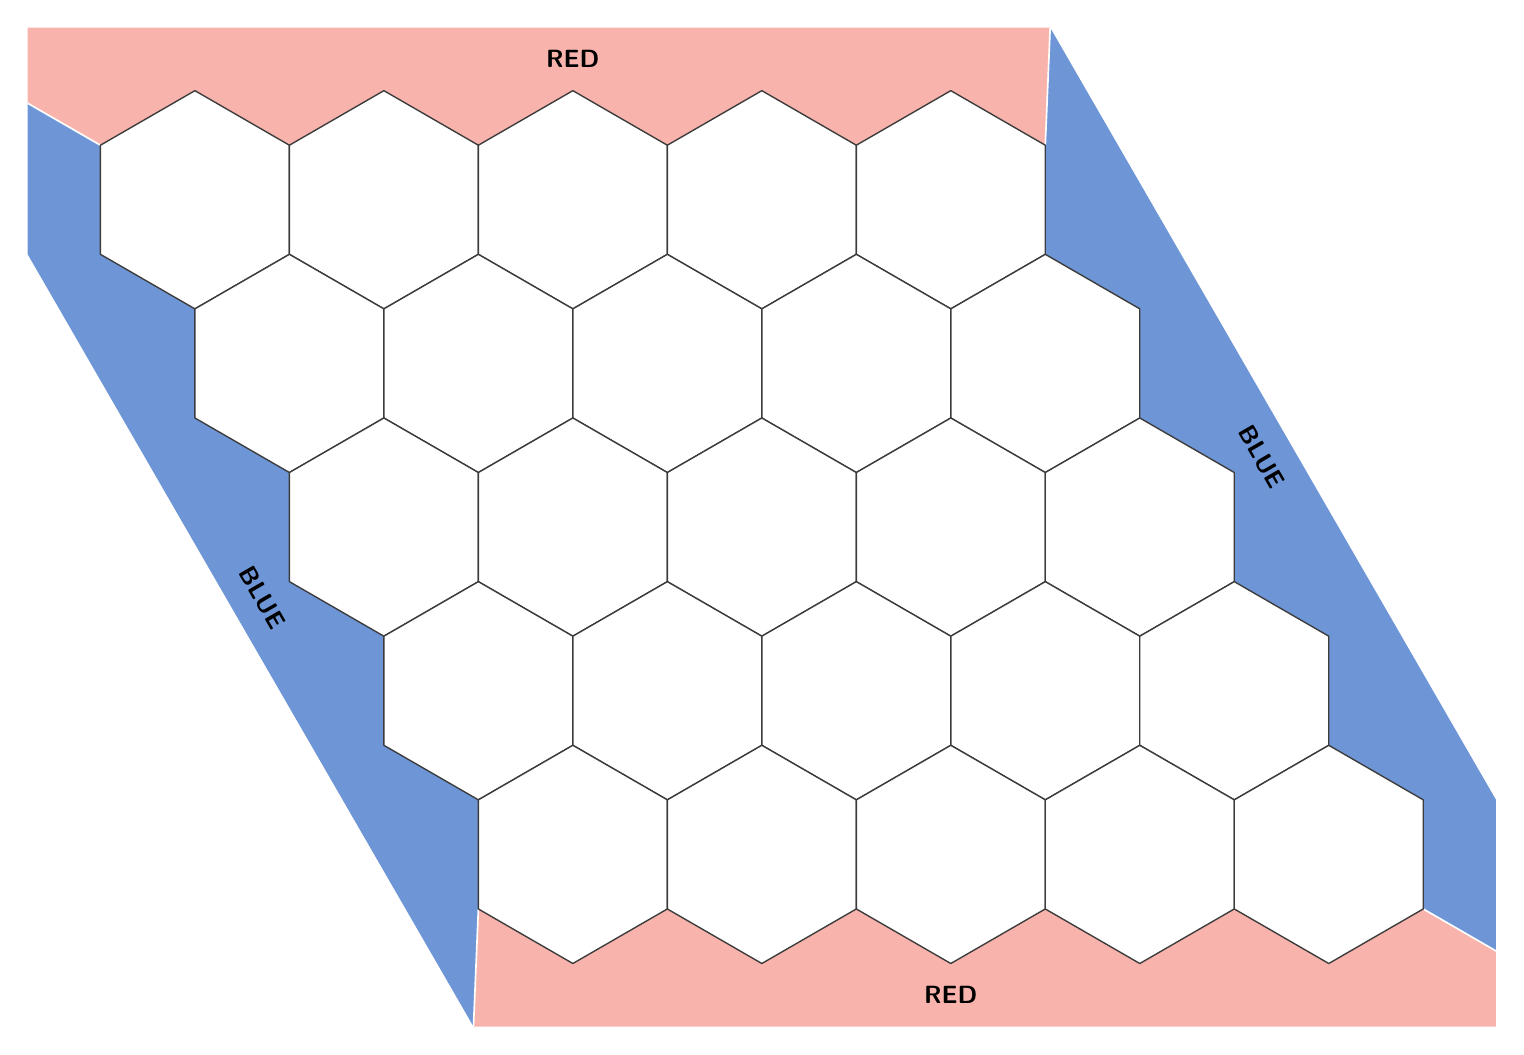
\begin{tikzpicture}[x=1.0mm,y=1.0mm,line join=round]
\begin{scope}
\clip (-21.238,-104.995) rectangle (165.238,21.856);
\fill[redtint] (-12.000,6.928) -- (0.000,13.856) -- (12.000,6.928) -- (24.000,13.856) -- (36.000,6.928) -- (48.000,13.856) -- (60.000,6.928) -- (72.000,13.856) -- (84.000,6.928) -- (96.000,13.856) -- (108.000,6.928) -- (108.619,21.856) -- (-37.856,21.856) -- cycle;
\fill[redtint] (156.000,-90.067) -- (144.000,-96.995) -- (132.000,-90.067) -- (120.000,-96.995) -- (108.000,-90.067) -- (96.000,-96.995) -- (84.000,-90.067) -- (72.000,-96.995) -- (60.000,-90.067) -- (48.000,-96.995) -- (36.000,-90.067) -- (35.381,-104.995) -- (181.856,-104.995) -- cycle;
\fill[bluetint] (36.000,-90.067) -- (36.000,-76.210) -- (24.000,-69.282) -- (24.000,-55.426) -- (12.000,-48.497) -- (12.000,-34.641) -- (0.000,-27.713) -- (-0.000,-13.856) -- (-12.000,-6.928) -- (-12.000,6.928) -- (-37.856,21.856) -- (35.381,-104.995) -- cycle;
\fill[bluetint] (108.000,6.928) -- (108.000,-6.928) -- (120.000,-13.856) -- (120.000,-27.713) -- (132.000,-34.641) -- (132.000,-48.497) -- (144.000,-55.426) -- (144.000,-69.282) -- (156.000,-76.210) -- (156.000,-90.067) -- (181.856,-104.995) -- (108.619,21.856) -- cycle;
\draw[white,line width=0.6pt] (-12.000,6.928) -- (-37.856,21.856);
\draw[white,line width=0.6pt] (108.000,6.928) -- (108.619,21.856);
\draw[white,line width=0.6pt] (156.000,-90.067) -- (181.856,-104.995);
\draw[white,line width=0.6pt] (36.000,-90.067) -- (35.381,-104.995);
\end{scope}
\node[font=\small\bfseries,text=black] at (48.000,17.856) {RED};
\node[font=\small\bfseries,text=black] at (96.000,-100.995) {RED};
\node[font=\small\bfseries,text=black,rotate=-60] at (8.536,-50.497) {BLUE};
\node[font=\small\bfseries,text=black,rotate=-60] at (135.464,-32.641) {BLUE};
\filldraw[fill=white,draw=gridline,line width=0.5pt] (12.000,6.928) -- (0.000,13.856) -- (-12.000,6.928) -- (-12.000,-6.928) -- (-0.000,-13.856) -- (12.000,-6.928) -- cycle;
\filldraw[fill=white,draw=gridline,line width=0.5pt] (36.000,6.928) -- (24.000,13.856) -- (12.000,6.928) -- (12.000,-6.928) -- (24.000,-13.856) -- (36.000,-6.928) -- cycle;
\filldraw[fill=white,draw=gridline,line width=0.5pt] (60.000,6.928) -- (48.000,13.856) -- (36.000,6.928) -- (36.000,-6.928) -- (48.000,-13.856) -- (60.000,-6.928) -- cycle;
\filldraw[fill=white,draw=gridline,line width=0.5pt] (84.000,6.928) -- (72.000,13.856) -- (60.000,6.928) -- (60.000,-6.928) -- (72.000,-13.856) -- (84.000,-6.928) -- cycle;
\filldraw[fill=white,draw=gridline,line width=0.5pt] (108.000,6.928) -- (96.000,13.856) -- (84.000,6.928) -- (84.000,-6.928) -- (96.000,-13.856) -- (108.000,-6.928) -- cycle;
\filldraw[fill=white,draw=gridline,line width=0.5pt] (24.000,-13.856) -- (12.000,-6.928) -- (-0.000,-13.856) -- (0.000,-27.713) -- (12.000,-34.641) -- (24.000,-27.713) -- cycle;
\filldraw[fill=white,draw=gridline,line width=0.5pt] (48.000,-13.856) -- (36.000,-6.928) -- (24.000,-13.856) -- (24.000,-27.713) -- (36.000,-34.641) -- (48.000,-27.713) -- cycle;
\filldraw[fill=white,draw=gridline,line width=0.5pt] (72.000,-13.856) -- (60.000,-6.928) -- (48.000,-13.856) -- (48.000,-27.713) -- (60.000,-34.641) -- (72.000,-27.713) -- cycle;
\filldraw[fill=white,draw=gridline,line width=0.5pt] (96.000,-13.856) -- (84.000,-6.928) -- (72.000,-13.856) -- (72.000,-27.713) -- (84.000,-34.641) -- (96.000,-27.713) -- cycle;
\filldraw[fill=white,draw=gridline,line width=0.5pt] (120.000,-13.856) -- (108.000,-6.928) -- (96.000,-13.856) -- (96.000,-27.713) -- (108.000,-34.641) -- (120.000,-27.713) -- cycle;
\filldraw[fill=white,draw=gridline,line width=0.5pt] (36.000,-34.641) -- (24.000,-27.713) -- (12.000,-34.641) -- (12.000,-48.497) -- (24.000,-55.426) -- (36.000,-48.497) -- cycle;
\filldraw[fill=white,draw=gridline,line width=0.5pt] (60.000,-34.641) -- (48.000,-27.713) -- (36.000,-34.641) -- (36.000,-48.497) -- (48.000,-55.426) -- (60.000,-48.497) -- cycle;
\filldraw[fill=white,draw=gridline,line width=0.5pt] (84.000,-34.641) -- (72.000,-27.713) -- (60.000,-34.641) -- (60.000,-48.497) -- (72.000,-55.426) -- (84.000,-48.497) -- cycle;
\filldraw[fill=white,draw=gridline,line width=0.5pt] (108.000,-34.641) -- (96.000,-27.713) -- (84.000,-34.641) -- (84.000,-48.497) -- (96.000,-55.426) -- (108.000,-48.497) -- cycle;
\filldraw[fill=white,draw=gridline,line width=0.5pt] (132.000,-34.641) -- (120.000,-27.713) -- (108.000,-34.641) -- (108.000,-48.497) -- (120.000,-55.426) -- (132.000,-48.497) -- cycle;
\filldraw[fill=white,draw=gridline,line width=0.5pt] (48.000,-55.426) -- (36.000,-48.497) -- (24.000,-55.426) -- (24.000,-69.282) -- (36.000,-76.210) -- (48.000,-69.282) -- cycle;
\filldraw[fill=white,draw=gridline,line width=0.5pt] (72.000,-55.426) -- (60.000,-48.497) -- (48.000,-55.426) -- (48.000,-69.282) -- (60.000,-76.210) -- (72.000,-69.282) -- cycle;
\filldraw[fill=white,draw=gridline,line width=0.5pt] (96.000,-55.426) -- (84.000,-48.497) -- (72.000,-55.426) -- (72.000,-69.282) -- (84.000,-76.210) -- (96.000,-69.282) -- cycle;
\filldraw[fill=white,draw=gridline,line width=0.5pt] (120.000,-55.426) -- (108.000,-48.497) -- (96.000,-55.426) -- (96.000,-69.282) -- (108.000,-76.210) -- (120.000,-69.282) -- cycle;
\filldraw[fill=white,draw=gridline,line width=0.5pt] (144.000,-55.426) -- (132.000,-48.497) -- (120.000,-55.426) -- (120.000,-69.282) -- (132.000,-76.210) -- (144.000,-69.282) -- cycle;
\filldraw[fill=white,draw=gridline,line width=0.5pt] (60.000,-76.210) -- (48.000,-69.282) -- (36.000,-76.210) -- (36.000,-90.067) -- (48.000,-96.995) -- (60.000,-90.067) -- cycle;
\filldraw[fill=white,draw=gridline,line width=0.5pt] (84.000,-76.210) -- (72.000,-69.282) -- (60.000,-76.210) -- (60.000,-90.067) -- (72.000,-96.995) -- (84.000,-90.067) -- cycle;
\filldraw[fill=white,draw=gridline,line width=0.5pt] (108.000,-76.210) -- (96.000,-69.282) -- (84.000,-76.210) -- (84.000,-90.067) -- (96.000,-96.995) -- (108.000,-90.067) -- cycle;
\filldraw[fill=white,draw=gridline,line width=0.5pt] (132.000,-76.210) -- (120.000,-69.282) -- (108.000,-76.210) -- (108.000,-90.067) -- (120.000,-96.995) -- (132.000,-90.067) -- cycle;
\filldraw[fill=white,draw=gridline,line width=0.5pt] (156.000,-76.210) -- (144.000,-69.282) -- (132.000,-76.210) -- (132.000,-90.067) -- (144.000,-96.995) -- (156.000,-90.067) -- cycle;
\end{tikzpicture}
\end{center}

\clearpage
\prob{3} Red goes first on this board. Find every hexagon where Red can put the first counter and then be sure to win, however Blue plays. Put an X on those hexagons on the small board.\par\vspace{2mm}\begin{center}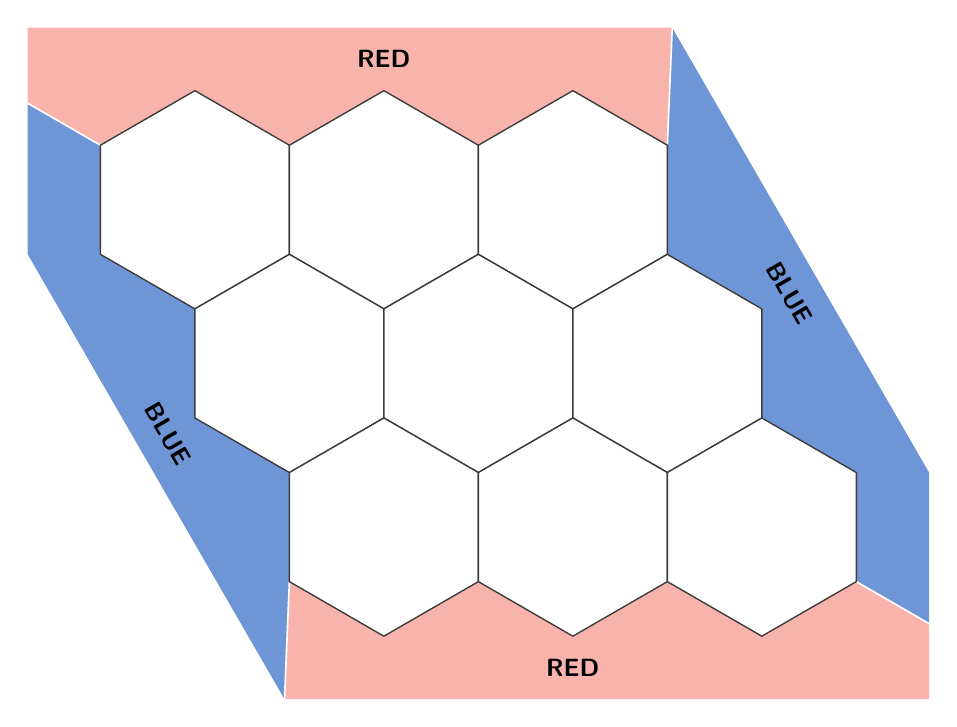
\begin{tikzpicture}[x=1.0mm,y=1.0mm,line join=round]
\begin{scope}
\clip (-21.238,-63.426) rectangle (93.238,21.856);
\fill[redtint] (-12.000,6.928) -- (0.000,13.856) -- (12.000,6.928) -- (24.000,13.856) -- (36.000,6.928) -- (48.000,13.856) -- (60.000,6.928) -- (60.619,21.856) -- (-37.856,21.856) -- cycle;
\fill[redtint] (84.000,-48.497) -- (72.000,-55.426) -- (60.000,-48.497) -- (48.000,-55.426) -- (36.000,-48.497) -- (24.000,-55.426) -- (12.000,-48.497) -- (11.381,-63.426) -- (109.856,-63.426) -- cycle;
\fill[bluetint] (12.000,-48.497) -- (12.000,-34.641) -- (0.000,-27.713) -- (-0.000,-13.856) -- (-12.000,-6.928) -- (-12.000,6.928) -- (-37.856,21.856) -- (11.381,-63.426) -- cycle;
\fill[bluetint] (60.000,6.928) -- (60.000,-6.928) -- (72.000,-13.856) -- (72.000,-27.713) -- (84.000,-34.641) -- (84.000,-48.497) -- (109.856,-63.426) -- (60.619,21.856) -- cycle;
\draw[white,line width=0.6pt] (-12.000,6.928) -- (-37.856,21.856);
\draw[white,line width=0.6pt] (60.000,6.928) -- (60.619,21.856);
\draw[white,line width=0.6pt] (84.000,-48.497) -- (109.856,-63.426);
\draw[white,line width=0.6pt] (12.000,-48.497) -- (11.381,-63.426);
\end{scope}
\node[font=\small\bfseries,text=black] at (24.000,17.856) {RED};
\node[font=\small\bfseries,text=black] at (48.000,-59.426) {RED};
\node[font=\small\bfseries,text=black,rotate=-60] at (-3.464,-29.713) {BLUE};
\node[font=\small\bfseries,text=black,rotate=-60] at (75.464,-11.856) {BLUE};
\filldraw[fill=white,draw=gridline,line width=0.5pt] (12.000,6.928) -- (0.000,13.856) -- (-12.000,6.928) -- (-12.000,-6.928) -- (-0.000,-13.856) -- (12.000,-6.928) -- cycle;
\filldraw[fill=white,draw=gridline,line width=0.5pt] (36.000,6.928) -- (24.000,13.856) -- (12.000,6.928) -- (12.000,-6.928) -- (24.000,-13.856) -- (36.000,-6.928) -- cycle;
\filldraw[fill=white,draw=gridline,line width=0.5pt] (60.000,6.928) -- (48.000,13.856) -- (36.000,6.928) -- (36.000,-6.928) -- (48.000,-13.856) -- (60.000,-6.928) -- cycle;
\filldraw[fill=white,draw=gridline,line width=0.5pt] (24.000,-13.856) -- (12.000,-6.928) -- (-0.000,-13.856) -- (0.000,-27.713) -- (12.000,-34.641) -- (24.000,-27.713) -- cycle;
\filldraw[fill=white,draw=gridline,line width=0.5pt] (48.000,-13.856) -- (36.000,-6.928) -- (24.000,-13.856) -- (24.000,-27.713) -- (36.000,-34.641) -- (48.000,-27.713) -- cycle;
\filldraw[fill=white,draw=gridline,line width=0.5pt] (72.000,-13.856) -- (60.000,-6.928) -- (48.000,-13.856) -- (48.000,-27.713) -- (60.000,-34.641) -- (72.000,-27.713) -- cycle;
\filldraw[fill=white,draw=gridline,line width=0.5pt] (36.000,-34.641) -- (24.000,-27.713) -- (12.000,-34.641) -- (12.000,-48.497) -- (24.000,-55.426) -- (36.000,-48.497) -- cycle;
\filldraw[fill=white,draw=gridline,line width=0.5pt] (60.000,-34.641) -- (48.000,-27.713) -- (36.000,-34.641) -- (36.000,-48.497) -- (48.000,-55.426) -- (60.000,-48.497) -- cycle;
\filldraw[fill=white,draw=gridline,line width=0.5pt] (84.000,-34.641) -- (72.000,-27.713) -- (60.000,-34.641) -- (60.000,-48.497) -- (72.000,-55.426) -- (84.000,-48.497) -- cycle;
\end{tikzpicture}\hspace{12mm}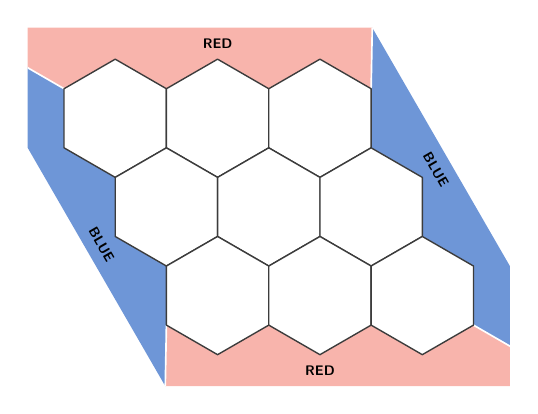
\begin{tikzpicture}[x=1.0mm,y=1.0mm,line join=round]
\begin{scope}
\clip (-11.119,-34.022) rectangle (50.119,11.506);
\fill[redtint] (-6.500,3.753) -- (0.000,7.506) -- (6.500,3.753) -- (13.000,7.506) -- (19.500,3.753) -- (26.000,7.506) -- (32.500,3.753) -- (32.643,11.506) -- (-19.928,11.506) -- cycle;
\fill[redtint] (45.500,-26.269) -- (39.000,-30.022) -- (32.500,-26.269) -- (26.000,-30.022) -- (19.500,-26.269) -- (13.000,-30.022) -- (6.500,-26.269) -- (6.357,-34.022) -- (58.928,-34.022) -- cycle;
\fill[bluetint] (6.500,-26.269) -- (6.500,-18.764) -- (0.000,-15.011) -- (-0.000,-7.506) -- (-6.500,-3.753) -- (-6.500,3.753) -- (-19.928,11.506) -- (6.357,-34.022) -- cycle;
\fill[bluetint] (32.500,3.753) -- (32.500,-3.753) -- (39.000,-7.506) -- (39.000,-15.011) -- (45.500,-18.764) -- (45.500,-26.269) -- (58.928,-34.022) -- (32.643,11.506) -- cycle;
\draw[white,line width=0.6pt] (-6.500,3.753) -- (-19.928,11.506);
\draw[white,line width=0.6pt] (32.500,3.753) -- (32.643,11.506);
\draw[white,line width=0.6pt] (45.500,-26.269) -- (58.928,-34.022);
\draw[white,line width=0.6pt] (6.500,-26.269) -- (6.357,-34.022);
\end{scope}
\node[font=\tiny\bfseries,text=black] at (13.000,9.506) {RED};
\node[font=\tiny\bfseries,text=black] at (26.000,-32.022) {RED};
\node[font=\tiny\bfseries,text=black,rotate=-60] at (-1.732,-16.011) {BLUE};
\node[font=\tiny\bfseries,text=black,rotate=-60] at (40.732,-6.506) {BLUE};
\filldraw[fill=white,draw=gridline,line width=0.5pt] (6.500,3.753) -- (0.000,7.506) -- (-6.500,3.753) -- (-6.500,-3.753) -- (-0.000,-7.506) -- (6.500,-3.753) -- cycle;
\filldraw[fill=white,draw=gridline,line width=0.5pt] (19.500,3.753) -- (13.000,7.506) -- (6.500,3.753) -- (6.500,-3.753) -- (13.000,-7.506) -- (19.500,-3.753) -- cycle;
\filldraw[fill=white,draw=gridline,line width=0.5pt] (32.500,3.753) -- (26.000,7.506) -- (19.500,3.753) -- (19.500,-3.753) -- (26.000,-7.506) -- (32.500,-3.753) -- cycle;
\filldraw[fill=white,draw=gridline,line width=0.5pt] (13.000,-7.506) -- (6.500,-3.753) -- (-0.000,-7.506) -- (0.000,-15.011) -- (6.500,-18.764) -- (13.000,-15.011) -- cycle;
\filldraw[fill=white,draw=gridline,line width=0.5pt] (26.000,-7.506) -- (19.500,-3.753) -- (13.000,-7.506) -- (13.000,-15.011) -- (19.500,-18.764) -- (26.000,-15.011) -- cycle;
\filldraw[fill=white,draw=gridline,line width=0.5pt] (39.000,-7.506) -- (32.500,-3.753) -- (26.000,-7.506) -- (26.000,-15.011) -- (32.500,-18.764) -- (39.000,-15.011) -- cycle;
\filldraw[fill=white,draw=gridline,line width=0.5pt] (19.500,-18.764) -- (13.000,-15.011) -- (6.500,-18.764) -- (6.500,-26.269) -- (13.000,-30.022) -- (19.500,-26.269) -- cycle;
\filldraw[fill=white,draw=gridline,line width=0.5pt] (32.500,-18.764) -- (26.000,-15.011) -- (19.500,-18.764) -- (19.500,-26.269) -- (26.000,-30.022) -- (32.500,-26.269) -- cycle;
\filldraw[fill=white,draw=gridline,line width=0.5pt] (45.500,-18.764) -- (39.000,-15.011) -- (32.500,-18.764) -- (32.500,-26.269) -- (39.000,-30.022) -- (45.500,-26.269) -- cycle;
\end{tikzpicture}\end{center}
\clearpage
\prob{4} On this board of squares, a chain is made of squares that each share a side with the next. Put a red or a blue counter on every square so that nobody wins. Next, count squares that touch only at a corner as touching too. Fill the board so that Red and Blue both win.
\begin{center}
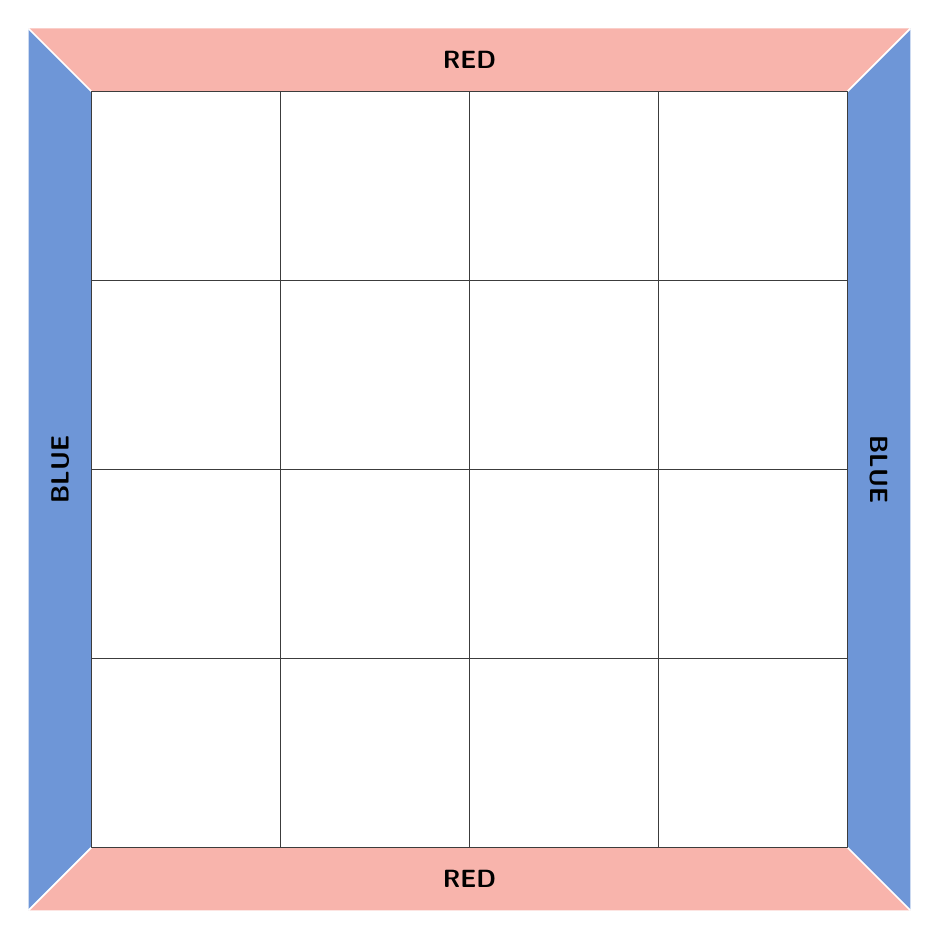
\begin{tikzpicture}[x=1mm,y=1mm,line join=round]
\fill[redtint] (0,96.0) -- (96.0,96.0) -- (104.0,104.0) -- (-8.0,104.0) -- cycle;
\fill[redtint] (0,0) -- (96.0,0) -- (104.0,-8.0) -- (-8.0,-8.0) -- cycle;
\fill[bluetint] (0,0) -- (0,96.0) -- (-8.0,104.0) -- (-8.0,-8.0) -- cycle;
\fill[bluetint] (96.0,0) -- (96.0,96.0) -- (104.0,104.0) -- (104.0,-8.0) -- cycle;
\draw[white,line width=0.6pt] (0,96.0) -- (-8.0,104.0);
\draw[white,line width=0.6pt] (96.0,96.0) -- (104.0,104.0);
\draw[white,line width=0.6pt] (0,0) -- (-8.0,-8.0);
\draw[white,line width=0.6pt] (96.0,0) -- (104.0,-8.0);
\node[font=\small\bfseries] at (48.0,100.0) {RED};
\node[font=\small\bfseries] at (48.0,-4.0) {RED};
\node[font=\small\bfseries,rotate=90] at (-4.0,48.0) {BLUE};
\node[font=\small\bfseries,rotate=-90] at (100.0,48.0) {BLUE};
\filldraw[fill=white,draw=gridline,line width=0.5pt] (0,0) rectangle (96.0,96.0);
\draw[gridline,line width=0.5pt] (24.0,0) -- (24.0,96.0);
\draw[gridline,line width=0.5pt] (0,24.0) -- (96.0,24.0);
\draw[gridline,line width=0.5pt] (48.0,0) -- (48.0,96.0);
\draw[gridline,line width=0.5pt] (0,48.0) -- (96.0,48.0);
\draw[gridline,line width=0.5pt] (72.0,0) -- (72.0,96.0);
\draw[gridline,line width=0.5pt] (0,72.0) -- (96.0,72.0);
\end{tikzpicture}
\end{center}
\vspace{6mm}

\prob{5} Explain why Red and Blue can never both have a winning chain on the same hexagon board.\par\vspace{11mm}\noindent\begin{tikzpicture}[x=1mm,y=1mm]
\draw[writeline,line width=0.5pt] (0,0.0) -- (189.5,0.0);
\draw[writeline,line width=0.5pt] (0,-10.0) -- (189.5,-10.0);
\draw[writeline,line width=0.5pt] (0,-20.0) -- (189.5,-20.0);
\draw[writeline,line width=0.5pt] (0,-30.0) -- (189.5,-30.0);
\draw[writeline,line width=0.5pt] (0,-40.0) -- (189.5,-40.0);
\end{tikzpicture}\par

\clearpage
\prob{6} On each board, start at the star and draw a path along the sides of the hexagons, always with red on one side of the path and blue on the other. The colored edges count as red and blue. Follow the path as far as it goes. Where does it end?
\begin{center}
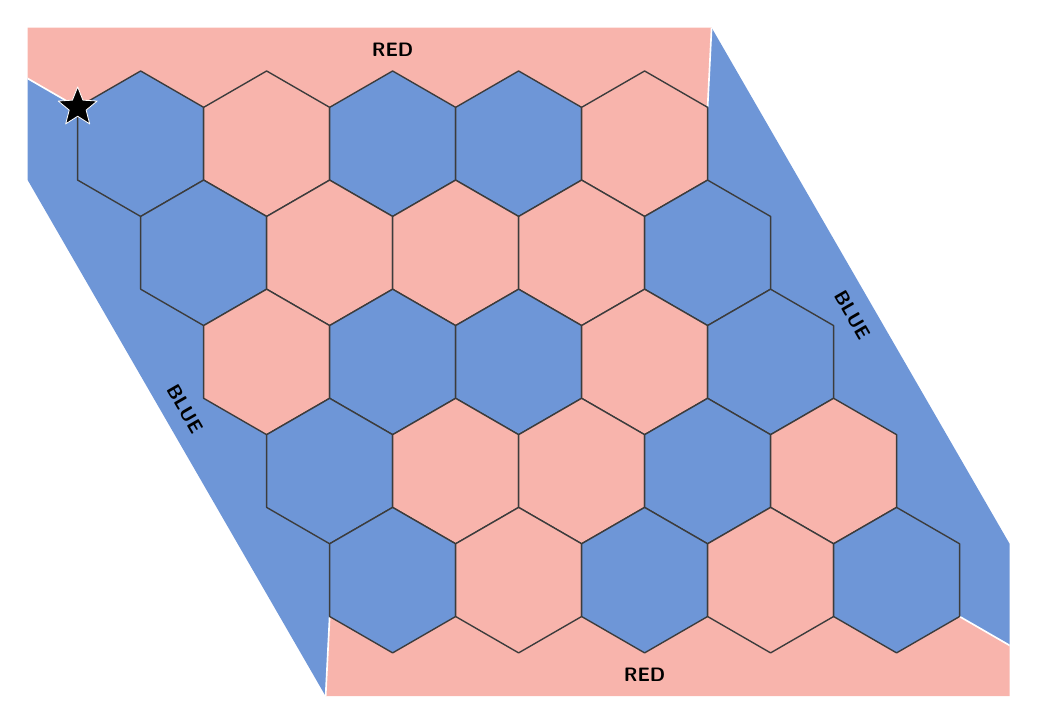
\begin{tikzpicture}[x=1.0mm,y=1.0mm,line join=round]
\begin{scope}
\clip (-14.351,-70.163) rectangle (110.351,14.738);
\fill[redtint] (-8.000,4.619) -- (0.000,9.238) -- (8.000,4.619) -- (16.000,9.238) -- (24.000,4.619) -- (32.000,9.238) -- (40.000,4.619) -- (48.000,9.238) -- (56.000,4.619) -- (64.000,9.238) -- (72.000,4.619) -- (72.509,14.738) -- (-25.526,14.738) -- cycle;
\fill[redtint] (104.000,-60.044) -- (96.000,-64.663) -- (88.000,-60.044) -- (80.000,-64.663) -- (72.000,-60.044) -- (64.000,-64.663) -- (56.000,-60.044) -- (48.000,-64.663) -- (40.000,-60.044) -- (32.000,-64.663) -- (24.000,-60.044) -- (23.491,-70.163) -- (121.526,-70.163) -- cycle;
\fill[bluetint] (24.000,-60.044) -- (24.000,-50.807) -- (16.000,-46.188) -- (16.000,-36.950) -- (8.000,-32.332) -- (8.000,-23.094) -- (0.000,-18.475) -- (-0.000,-9.238) -- (-8.000,-4.619) -- (-8.000,4.619) -- (-25.526,14.738) -- (23.491,-70.163) -- cycle;
\fill[bluetint] (72.000,4.619) -- (72.000,-4.619) -- (80.000,-9.238) -- (80.000,-18.475) -- (88.000,-23.094) -- (88.000,-32.332) -- (96.000,-36.950) -- (96.000,-46.188) -- (104.000,-50.807) -- (104.000,-60.044) -- (121.526,-70.163) -- (72.509,14.738) -- cycle;
\draw[white,line width=0.6pt] (-8.000,4.619) -- (-25.526,14.738);
\draw[white,line width=0.6pt] (72.000,4.619) -- (72.509,14.738);
\draw[white,line width=0.6pt] (104.000,-60.044) -- (121.526,-70.163);
\draw[white,line width=0.6pt] (24.000,-60.044) -- (23.491,-70.163);
\end{scope}
\node[font=\scriptsize\bfseries,text=black] at (32.000,11.988) {RED};
\node[font=\scriptsize\bfseries,text=black] at (64.000,-67.413) {RED};
\node[font=\scriptsize\bfseries,text=black,rotate=-60] at (5.618,-33.707) {BLUE};
\node[font=\scriptsize\bfseries,text=black,rotate=-60] at (90.382,-21.719) {BLUE};
\filldraw[fill=bluetint,draw=gridline,line width=0.5pt] (8.000,4.619) -- (0.000,9.238) -- (-8.000,4.619) -- (-8.000,-4.619) -- (-0.000,-9.238) -- (8.000,-4.619) -- cycle;
\filldraw[fill=redtint,draw=gridline,line width=0.5pt] (24.000,4.619) -- (16.000,9.238) -- (8.000,4.619) -- (8.000,-4.619) -- (16.000,-9.238) -- (24.000,-4.619) -- cycle;
\filldraw[fill=bluetint,draw=gridline,line width=0.5pt] (40.000,4.619) -- (32.000,9.238) -- (24.000,4.619) -- (24.000,-4.619) -- (32.000,-9.238) -- (40.000,-4.619) -- cycle;
\filldraw[fill=bluetint,draw=gridline,line width=0.5pt] (56.000,4.619) -- (48.000,9.238) -- (40.000,4.619) -- (40.000,-4.619) -- (48.000,-9.238) -- (56.000,-4.619) -- cycle;
\filldraw[fill=redtint,draw=gridline,line width=0.5pt] (72.000,4.619) -- (64.000,9.238) -- (56.000,4.619) -- (56.000,-4.619) -- (64.000,-9.238) -- (72.000,-4.619) -- cycle;
\filldraw[fill=bluetint,draw=gridline,line width=0.5pt] (16.000,-9.238) -- (8.000,-4.619) -- (-0.000,-9.238) -- (0.000,-18.475) -- (8.000,-23.094) -- (16.000,-18.475) -- cycle;
\filldraw[fill=redtint,draw=gridline,line width=0.5pt] (32.000,-9.238) -- (24.000,-4.619) -- (16.000,-9.238) -- (16.000,-18.475) -- (24.000,-23.094) -- (32.000,-18.475) -- cycle;
\filldraw[fill=redtint,draw=gridline,line width=0.5pt] (48.000,-9.238) -- (40.000,-4.619) -- (32.000,-9.238) -- (32.000,-18.475) -- (40.000,-23.094) -- (48.000,-18.475) -- cycle;
\filldraw[fill=redtint,draw=gridline,line width=0.5pt] (64.000,-9.238) -- (56.000,-4.619) -- (48.000,-9.238) -- (48.000,-18.475) -- (56.000,-23.094) -- (64.000,-18.475) -- cycle;
\filldraw[fill=bluetint,draw=gridline,line width=0.5pt] (80.000,-9.238) -- (72.000,-4.619) -- (64.000,-9.238) -- (64.000,-18.475) -- (72.000,-23.094) -- (80.000,-18.475) -- cycle;
\filldraw[fill=redtint,draw=gridline,line width=0.5pt] (24.000,-23.094) -- (16.000,-18.475) -- (8.000,-23.094) -- (8.000,-32.332) -- (16.000,-36.950) -- (24.000,-32.332) -- cycle;
\filldraw[fill=bluetint,draw=gridline,line width=0.5pt] (40.000,-23.094) -- (32.000,-18.475) -- (24.000,-23.094) -- (24.000,-32.332) -- (32.000,-36.950) -- (40.000,-32.332) -- cycle;
\filldraw[fill=bluetint,draw=gridline,line width=0.5pt] (56.000,-23.094) -- (48.000,-18.475) -- (40.000,-23.094) -- (40.000,-32.332) -- (48.000,-36.950) -- (56.000,-32.332) -- cycle;
\filldraw[fill=redtint,draw=gridline,line width=0.5pt] (72.000,-23.094) -- (64.000,-18.475) -- (56.000,-23.094) -- (56.000,-32.332) -- (64.000,-36.950) -- (72.000,-32.332) -- cycle;
\filldraw[fill=bluetint,draw=gridline,line width=0.5pt] (88.000,-23.094) -- (80.000,-18.475) -- (72.000,-23.094) -- (72.000,-32.332) -- (80.000,-36.950) -- (88.000,-32.332) -- cycle;
\filldraw[fill=bluetint,draw=gridline,line width=0.5pt] (32.000,-36.950) -- (24.000,-32.332) -- (16.000,-36.950) -- (16.000,-46.188) -- (24.000,-50.807) -- (32.000,-46.188) -- cycle;
\filldraw[fill=redtint,draw=gridline,line width=0.5pt] (48.000,-36.950) -- (40.000,-32.332) -- (32.000,-36.950) -- (32.000,-46.188) -- (40.000,-50.807) -- (48.000,-46.188) -- cycle;
\filldraw[fill=redtint,draw=gridline,line width=0.5pt] (64.000,-36.950) -- (56.000,-32.332) -- (48.000,-36.950) -- (48.000,-46.188) -- (56.000,-50.807) -- (64.000,-46.188) -- cycle;
\filldraw[fill=bluetint,draw=gridline,line width=0.5pt] (80.000,-36.950) -- (72.000,-32.332) -- (64.000,-36.950) -- (64.000,-46.188) -- (72.000,-50.807) -- (80.000,-46.188) -- cycle;
\filldraw[fill=redtint,draw=gridline,line width=0.5pt] (96.000,-36.950) -- (88.000,-32.332) -- (80.000,-36.950) -- (80.000,-46.188) -- (88.000,-50.807) -- (96.000,-46.188) -- cycle;
\filldraw[fill=bluetint,draw=gridline,line width=0.5pt] (40.000,-50.807) -- (32.000,-46.188) -- (24.000,-50.807) -- (24.000,-60.044) -- (32.000,-64.663) -- (40.000,-60.044) -- cycle;
\filldraw[fill=redtint,draw=gridline,line width=0.5pt] (56.000,-50.807) -- (48.000,-46.188) -- (40.000,-50.807) -- (40.000,-60.044) -- (48.000,-64.663) -- (56.000,-60.044) -- cycle;
\filldraw[fill=bluetint,draw=gridline,line width=0.5pt] (72.000,-50.807) -- (64.000,-46.188) -- (56.000,-50.807) -- (56.000,-60.044) -- (64.000,-64.663) -- (72.000,-60.044) -- cycle;
\filldraw[fill=redtint,draw=gridline,line width=0.5pt] (88.000,-50.807) -- (80.000,-46.188) -- (72.000,-50.807) -- (72.000,-60.044) -- (80.000,-64.663) -- (88.000,-60.044) -- cycle;
\filldraw[fill=bluetint,draw=gridline,line width=0.5pt] (104.000,-50.807) -- (96.000,-46.188) -- (88.000,-50.807) -- (88.000,-60.044) -- (96.000,-64.663) -- (104.000,-60.044) -- cycle;
\node[star,star points=5,star point ratio=2.3,fill=black,draw=white,line width=0.3pt,inner sep=0pt,minimum size=5.2mm] at (-8.000,4.619) {};
\end{tikzpicture}
\end{center}
\vspace{4mm}

\begin{center}
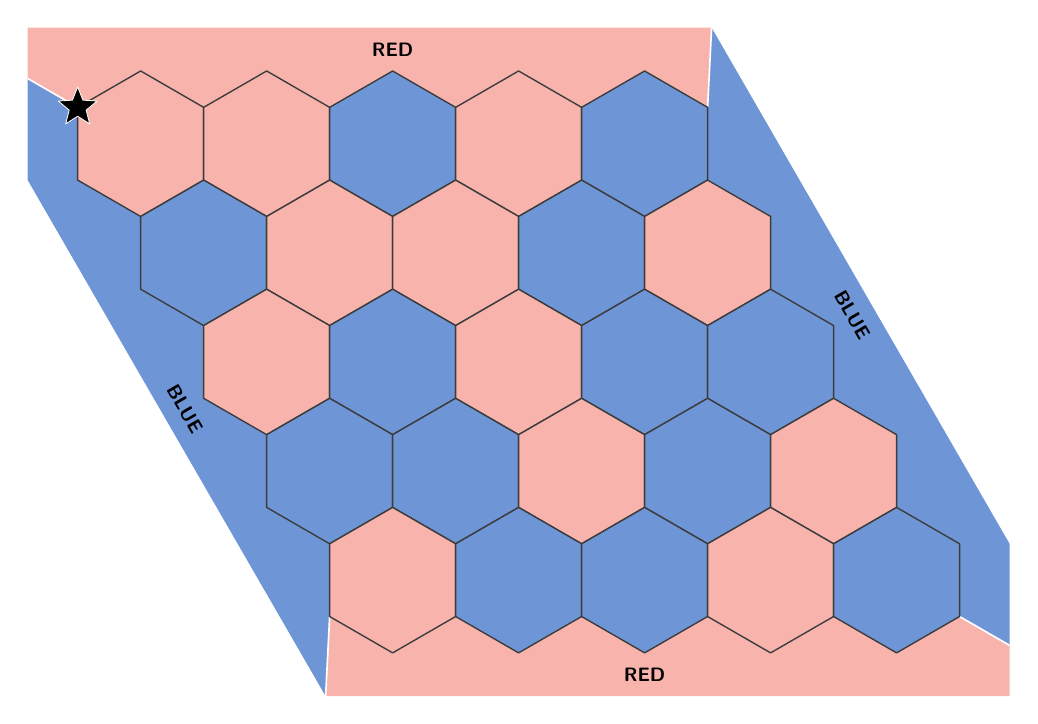
\begin{tikzpicture}[x=1.0mm,y=1.0mm,line join=round]
\begin{scope}
\clip (-14.351,-70.163) rectangle (110.351,14.738);
\fill[redtint] (-8.000,4.619) -- (0.000,9.238) -- (8.000,4.619) -- (16.000,9.238) -- (24.000,4.619) -- (32.000,9.238) -- (40.000,4.619) -- (48.000,9.238) -- (56.000,4.619) -- (64.000,9.238) -- (72.000,4.619) -- (72.509,14.738) -- (-25.526,14.738) -- cycle;
\fill[redtint] (104.000,-60.044) -- (96.000,-64.663) -- (88.000,-60.044) -- (80.000,-64.663) -- (72.000,-60.044) -- (64.000,-64.663) -- (56.000,-60.044) -- (48.000,-64.663) -- (40.000,-60.044) -- (32.000,-64.663) -- (24.000,-60.044) -- (23.491,-70.163) -- (121.526,-70.163) -- cycle;
\fill[bluetint] (24.000,-60.044) -- (24.000,-50.807) -- (16.000,-46.188) -- (16.000,-36.950) -- (8.000,-32.332) -- (8.000,-23.094) -- (0.000,-18.475) -- (-0.000,-9.238) -- (-8.000,-4.619) -- (-8.000,4.619) -- (-25.526,14.738) -- (23.491,-70.163) -- cycle;
\fill[bluetint] (72.000,4.619) -- (72.000,-4.619) -- (80.000,-9.238) -- (80.000,-18.475) -- (88.000,-23.094) -- (88.000,-32.332) -- (96.000,-36.950) -- (96.000,-46.188) -- (104.000,-50.807) -- (104.000,-60.044) -- (121.526,-70.163) -- (72.509,14.738) -- cycle;
\draw[white,line width=0.6pt] (-8.000,4.619) -- (-25.526,14.738);
\draw[white,line width=0.6pt] (72.000,4.619) -- (72.509,14.738);
\draw[white,line width=0.6pt] (104.000,-60.044) -- (121.526,-70.163);
\draw[white,line width=0.6pt] (24.000,-60.044) -- (23.491,-70.163);
\end{scope}
\node[font=\scriptsize\bfseries,text=black] at (32.000,11.988) {RED};
\node[font=\scriptsize\bfseries,text=black] at (64.000,-67.413) {RED};
\node[font=\scriptsize\bfseries,text=black,rotate=-60] at (5.618,-33.707) {BLUE};
\node[font=\scriptsize\bfseries,text=black,rotate=-60] at (90.382,-21.719) {BLUE};
\filldraw[fill=redtint,draw=gridline,line width=0.5pt] (8.000,4.619) -- (0.000,9.238) -- (-8.000,4.619) -- (-8.000,-4.619) -- (-0.000,-9.238) -- (8.000,-4.619) -- cycle;
\filldraw[fill=redtint,draw=gridline,line width=0.5pt] (24.000,4.619) -- (16.000,9.238) -- (8.000,4.619) -- (8.000,-4.619) -- (16.000,-9.238) -- (24.000,-4.619) -- cycle;
\filldraw[fill=bluetint,draw=gridline,line width=0.5pt] (40.000,4.619) -- (32.000,9.238) -- (24.000,4.619) -- (24.000,-4.619) -- (32.000,-9.238) -- (40.000,-4.619) -- cycle;
\filldraw[fill=redtint,draw=gridline,line width=0.5pt] (56.000,4.619) -- (48.000,9.238) -- (40.000,4.619) -- (40.000,-4.619) -- (48.000,-9.238) -- (56.000,-4.619) -- cycle;
\filldraw[fill=bluetint,draw=gridline,line width=0.5pt] (72.000,4.619) -- (64.000,9.238) -- (56.000,4.619) -- (56.000,-4.619) -- (64.000,-9.238) -- (72.000,-4.619) -- cycle;
\filldraw[fill=bluetint,draw=gridline,line width=0.5pt] (16.000,-9.238) -- (8.000,-4.619) -- (-0.000,-9.238) -- (0.000,-18.475) -- (8.000,-23.094) -- (16.000,-18.475) -- cycle;
\filldraw[fill=redtint,draw=gridline,line width=0.5pt] (32.000,-9.238) -- (24.000,-4.619) -- (16.000,-9.238) -- (16.000,-18.475) -- (24.000,-23.094) -- (32.000,-18.475) -- cycle;
\filldraw[fill=redtint,draw=gridline,line width=0.5pt] (48.000,-9.238) -- (40.000,-4.619) -- (32.000,-9.238) -- (32.000,-18.475) -- (40.000,-23.094) -- (48.000,-18.475) -- cycle;
\filldraw[fill=bluetint,draw=gridline,line width=0.5pt] (64.000,-9.238) -- (56.000,-4.619) -- (48.000,-9.238) -- (48.000,-18.475) -- (56.000,-23.094) -- (64.000,-18.475) -- cycle;
\filldraw[fill=redtint,draw=gridline,line width=0.5pt] (80.000,-9.238) -- (72.000,-4.619) -- (64.000,-9.238) -- (64.000,-18.475) -- (72.000,-23.094) -- (80.000,-18.475) -- cycle;
\filldraw[fill=redtint,draw=gridline,line width=0.5pt] (24.000,-23.094) -- (16.000,-18.475) -- (8.000,-23.094) -- (8.000,-32.332) -- (16.000,-36.950) -- (24.000,-32.332) -- cycle;
\filldraw[fill=bluetint,draw=gridline,line width=0.5pt] (40.000,-23.094) -- (32.000,-18.475) -- (24.000,-23.094) -- (24.000,-32.332) -- (32.000,-36.950) -- (40.000,-32.332) -- cycle;
\filldraw[fill=redtint,draw=gridline,line width=0.5pt] (56.000,-23.094) -- (48.000,-18.475) -- (40.000,-23.094) -- (40.000,-32.332) -- (48.000,-36.950) -- (56.000,-32.332) -- cycle;
\filldraw[fill=bluetint,draw=gridline,line width=0.5pt] (72.000,-23.094) -- (64.000,-18.475) -- (56.000,-23.094) -- (56.000,-32.332) -- (64.000,-36.950) -- (72.000,-32.332) -- cycle;
\filldraw[fill=bluetint,draw=gridline,line width=0.5pt] (88.000,-23.094) -- (80.000,-18.475) -- (72.000,-23.094) -- (72.000,-32.332) -- (80.000,-36.950) -- (88.000,-32.332) -- cycle;
\filldraw[fill=bluetint,draw=gridline,line width=0.5pt] (32.000,-36.950) -- (24.000,-32.332) -- (16.000,-36.950) -- (16.000,-46.188) -- (24.000,-50.807) -- (32.000,-46.188) -- cycle;
\filldraw[fill=bluetint,draw=gridline,line width=0.5pt] (48.000,-36.950) -- (40.000,-32.332) -- (32.000,-36.950) -- (32.000,-46.188) -- (40.000,-50.807) -- (48.000,-46.188) -- cycle;
\filldraw[fill=redtint,draw=gridline,line width=0.5pt] (64.000,-36.950) -- (56.000,-32.332) -- (48.000,-36.950) -- (48.000,-46.188) -- (56.000,-50.807) -- (64.000,-46.188) -- cycle;
\filldraw[fill=bluetint,draw=gridline,line width=0.5pt] (80.000,-36.950) -- (72.000,-32.332) -- (64.000,-36.950) -- (64.000,-46.188) -- (72.000,-50.807) -- (80.000,-46.188) -- cycle;
\filldraw[fill=redtint,draw=gridline,line width=0.5pt] (96.000,-36.950) -- (88.000,-32.332) -- (80.000,-36.950) -- (80.000,-46.188) -- (88.000,-50.807) -- (96.000,-46.188) -- cycle;
\filldraw[fill=redtint,draw=gridline,line width=0.5pt] (40.000,-50.807) -- (32.000,-46.188) -- (24.000,-50.807) -- (24.000,-60.044) -- (32.000,-64.663) -- (40.000,-60.044) -- cycle;
\filldraw[fill=bluetint,draw=gridline,line width=0.5pt] (56.000,-50.807) -- (48.000,-46.188) -- (40.000,-50.807) -- (40.000,-60.044) -- (48.000,-64.663) -- (56.000,-60.044) -- cycle;
\filldraw[fill=bluetint,draw=gridline,line width=0.5pt] (72.000,-50.807) -- (64.000,-46.188) -- (56.000,-50.807) -- (56.000,-60.044) -- (64.000,-64.663) -- (72.000,-60.044) -- cycle;
\filldraw[fill=redtint,draw=gridline,line width=0.5pt] (88.000,-50.807) -- (80.000,-46.188) -- (72.000,-50.807) -- (72.000,-60.044) -- (80.000,-64.663) -- (88.000,-60.044) -- cycle;
\filldraw[fill=bluetint,draw=gridline,line width=0.5pt] (104.000,-50.807) -- (96.000,-46.188) -- (88.000,-50.807) -- (88.000,-60.044) -- (96.000,-64.663) -- (104.000,-60.044) -- cycle;
\node[star,star points=5,star point ratio=2.3,fill=black,draw=white,line width=0.3pt,inner sep=0pt,minimum size=5.2mm] at (-8.000,4.619) {};
\end{tikzpicture}
\end{center}

\clearpage
\prob{7} Color every hexagon on these boards red or blue, any way you like. Then draw the path from the star on each board, as in Problem 6. Can a path end anywhere other than the places where the paths in Problem 6 ended?\par\vspace{2mm}\begin{center}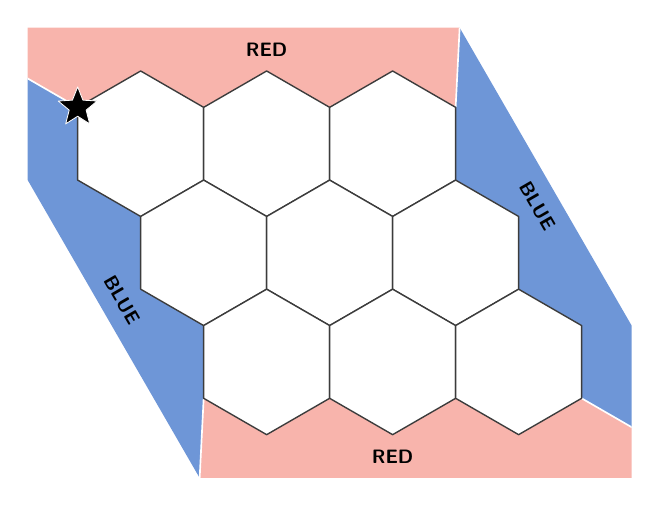
\begin{tikzpicture}[x=1.0mm,y=1.0mm,line join=round]
\begin{scope}
\clip (-14.351,-42.450) rectangle (62.351,14.738);
\fill[redtint] (-8.000,4.619) -- (0.000,9.238) -- (8.000,4.619) -- (16.000,9.238) -- (24.000,4.619) -- (32.000,9.238) -- (40.000,4.619) -- (40.509,14.738) -- (-25.526,14.738) -- cycle;
\fill[redtint] (56.000,-32.332) -- (48.000,-36.950) -- (40.000,-32.332) -- (32.000,-36.950) -- (24.000,-32.332) -- (16.000,-36.950) -- (8.000,-32.332) -- (7.491,-42.450) -- (73.526,-42.450) -- cycle;
\fill[bluetint] (8.000,-32.332) -- (8.000,-23.094) -- (0.000,-18.475) -- (-0.000,-9.238) -- (-8.000,-4.619) -- (-8.000,4.619) -- (-25.526,14.738) -- (7.491,-42.450) -- cycle;
\fill[bluetint] (40.000,4.619) -- (40.000,-4.619) -- (48.000,-9.238) -- (48.000,-18.475) -- (56.000,-23.094) -- (56.000,-32.332) -- (73.526,-42.450) -- (40.509,14.738) -- cycle;
\draw[white,line width=0.6pt] (-8.000,4.619) -- (-25.526,14.738);
\draw[white,line width=0.6pt] (40.000,4.619) -- (40.509,14.738);
\draw[white,line width=0.6pt] (56.000,-32.332) -- (73.526,-42.450);
\draw[white,line width=0.6pt] (8.000,-32.332) -- (7.491,-42.450);
\end{scope}
\node[font=\scriptsize\bfseries,text=black] at (16.000,11.988) {RED};
\node[font=\scriptsize\bfseries,text=black] at (32.000,-39.700) {RED};
\node[font=\scriptsize\bfseries,text=black,rotate=-60] at (-2.382,-19.850) {BLUE};
\node[font=\scriptsize\bfseries,text=black,rotate=-60] at (50.382,-7.863) {BLUE};
\filldraw[fill=white,draw=gridline,line width=0.5pt] (8.000,4.619) -- (0.000,9.238) -- (-8.000,4.619) -- (-8.000,-4.619) -- (-0.000,-9.238) -- (8.000,-4.619) -- cycle;
\filldraw[fill=white,draw=gridline,line width=0.5pt] (24.000,4.619) -- (16.000,9.238) -- (8.000,4.619) -- (8.000,-4.619) -- (16.000,-9.238) -- (24.000,-4.619) -- cycle;
\filldraw[fill=white,draw=gridline,line width=0.5pt] (40.000,4.619) -- (32.000,9.238) -- (24.000,4.619) -- (24.000,-4.619) -- (32.000,-9.238) -- (40.000,-4.619) -- cycle;
\filldraw[fill=white,draw=gridline,line width=0.5pt] (16.000,-9.238) -- (8.000,-4.619) -- (-0.000,-9.238) -- (0.000,-18.475) -- (8.000,-23.094) -- (16.000,-18.475) -- cycle;
\filldraw[fill=white,draw=gridline,line width=0.5pt] (32.000,-9.238) -- (24.000,-4.619) -- (16.000,-9.238) -- (16.000,-18.475) -- (24.000,-23.094) -- (32.000,-18.475) -- cycle;
\filldraw[fill=white,draw=gridline,line width=0.5pt] (48.000,-9.238) -- (40.000,-4.619) -- (32.000,-9.238) -- (32.000,-18.475) -- (40.000,-23.094) -- (48.000,-18.475) -- cycle;
\filldraw[fill=white,draw=gridline,line width=0.5pt] (24.000,-23.094) -- (16.000,-18.475) -- (8.000,-23.094) -- (8.000,-32.332) -- (16.000,-36.950) -- (24.000,-32.332) -- cycle;
\filldraw[fill=white,draw=gridline,line width=0.5pt] (40.000,-23.094) -- (32.000,-18.475) -- (24.000,-23.094) -- (24.000,-32.332) -- (32.000,-36.950) -- (40.000,-32.332) -- cycle;
\filldraw[fill=white,draw=gridline,line width=0.5pt] (56.000,-23.094) -- (48.000,-18.475) -- (40.000,-23.094) -- (40.000,-32.332) -- (48.000,-36.950) -- (56.000,-32.332) -- cycle;
\node[star,star points=5,star point ratio=2.3,fill=black,draw=white,line width=0.3pt,inner sep=0pt,minimum size=5.2mm] at (-8.000,4.619) {};
\end{tikzpicture}\hspace{10mm}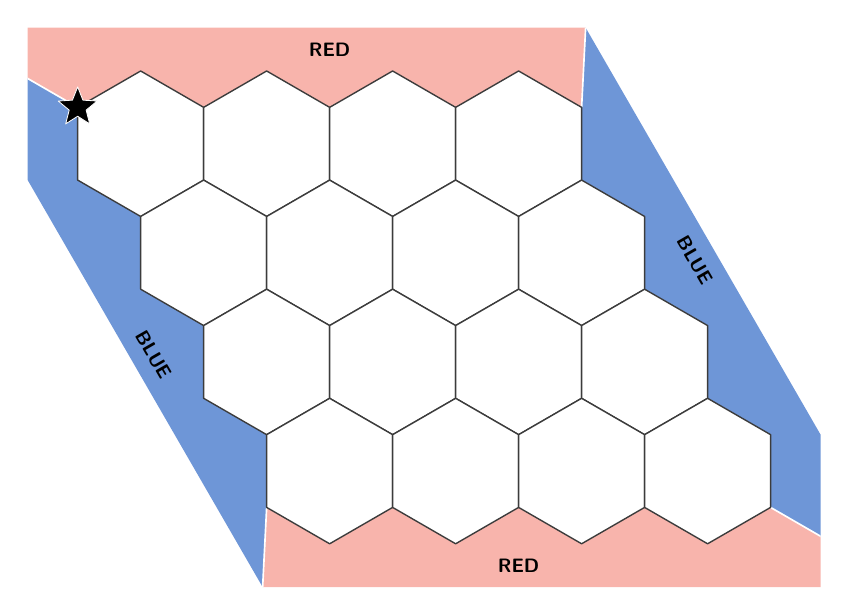
\begin{tikzpicture}[x=1.0mm,y=1.0mm,line join=round]
\begin{scope}
\clip (-14.351,-56.307) rectangle (86.351,14.738);
\fill[redtint] (-8.000,4.619) -- (0.000,9.238) -- (8.000,4.619) -- (16.000,9.238) -- (24.000,4.619) -- (32.000,9.238) -- (40.000,4.619) -- (48.000,9.238) -- (56.000,4.619) -- (56.509,14.738) -- (-25.526,14.738) -- cycle;
\fill[redtint] (80.000,-46.188) -- (72.000,-50.807) -- (64.000,-46.188) -- (56.000,-50.807) -- (48.000,-46.188) -- (40.000,-50.807) -- (32.000,-46.188) -- (24.000,-50.807) -- (16.000,-46.188) -- (15.491,-56.307) -- (97.526,-56.307) -- cycle;
\fill[bluetint] (16.000,-46.188) -- (16.000,-36.950) -- (8.000,-32.332) -- (8.000,-23.094) -- (0.000,-18.475) -- (-0.000,-9.238) -- (-8.000,-4.619) -- (-8.000,4.619) -- (-25.526,14.738) -- (15.491,-56.307) -- cycle;
\fill[bluetint] (56.000,4.619) -- (56.000,-4.619) -- (64.000,-9.238) -- (64.000,-18.475) -- (72.000,-23.094) -- (72.000,-32.332) -- (80.000,-36.950) -- (80.000,-46.188) -- (97.526,-56.307) -- (56.509,14.738) -- cycle;
\draw[white,line width=0.6pt] (-8.000,4.619) -- (-25.526,14.738);
\draw[white,line width=0.6pt] (56.000,4.619) -- (56.509,14.738);
\draw[white,line width=0.6pt] (80.000,-46.188) -- (97.526,-56.307);
\draw[white,line width=0.6pt] (16.000,-46.188) -- (15.491,-56.307);
\end{scope}
\node[font=\scriptsize\bfseries,text=black] at (24.000,11.988) {RED};
\node[font=\scriptsize\bfseries,text=black] at (48.000,-53.557) {RED};
\node[font=\scriptsize\bfseries,text=black,rotate=-60] at (1.618,-26.778) {BLUE};
\node[font=\scriptsize\bfseries,text=black,rotate=-60] at (70.382,-14.791) {BLUE};
\filldraw[fill=white,draw=gridline,line width=0.5pt] (8.000,4.619) -- (0.000,9.238) -- (-8.000,4.619) -- (-8.000,-4.619) -- (-0.000,-9.238) -- (8.000,-4.619) -- cycle;
\filldraw[fill=white,draw=gridline,line width=0.5pt] (24.000,4.619) -- (16.000,9.238) -- (8.000,4.619) -- (8.000,-4.619) -- (16.000,-9.238) -- (24.000,-4.619) -- cycle;
\filldraw[fill=white,draw=gridline,line width=0.5pt] (40.000,4.619) -- (32.000,9.238) -- (24.000,4.619) -- (24.000,-4.619) -- (32.000,-9.238) -- (40.000,-4.619) -- cycle;
\filldraw[fill=white,draw=gridline,line width=0.5pt] (56.000,4.619) -- (48.000,9.238) -- (40.000,4.619) -- (40.000,-4.619) -- (48.000,-9.238) -- (56.000,-4.619) -- cycle;
\filldraw[fill=white,draw=gridline,line width=0.5pt] (16.000,-9.238) -- (8.000,-4.619) -- (-0.000,-9.238) -- (0.000,-18.475) -- (8.000,-23.094) -- (16.000,-18.475) -- cycle;
\filldraw[fill=white,draw=gridline,line width=0.5pt] (32.000,-9.238) -- (24.000,-4.619) -- (16.000,-9.238) -- (16.000,-18.475) -- (24.000,-23.094) -- (32.000,-18.475) -- cycle;
\filldraw[fill=white,draw=gridline,line width=0.5pt] (48.000,-9.238) -- (40.000,-4.619) -- (32.000,-9.238) -- (32.000,-18.475) -- (40.000,-23.094) -- (48.000,-18.475) -- cycle;
\filldraw[fill=white,draw=gridline,line width=0.5pt] (64.000,-9.238) -- (56.000,-4.619) -- (48.000,-9.238) -- (48.000,-18.475) -- (56.000,-23.094) -- (64.000,-18.475) -- cycle;
\filldraw[fill=white,draw=gridline,line width=0.5pt] (24.000,-23.094) -- (16.000,-18.475) -- (8.000,-23.094) -- (8.000,-32.332) -- (16.000,-36.950) -- (24.000,-32.332) -- cycle;
\filldraw[fill=white,draw=gridline,line width=0.5pt] (40.000,-23.094) -- (32.000,-18.475) -- (24.000,-23.094) -- (24.000,-32.332) -- (32.000,-36.950) -- (40.000,-32.332) -- cycle;
\filldraw[fill=white,draw=gridline,line width=0.5pt] (56.000,-23.094) -- (48.000,-18.475) -- (40.000,-23.094) -- (40.000,-32.332) -- (48.000,-36.950) -- (56.000,-32.332) -- cycle;
\filldraw[fill=white,draw=gridline,line width=0.5pt] (72.000,-23.094) -- (64.000,-18.475) -- (56.000,-23.094) -- (56.000,-32.332) -- (64.000,-36.950) -- (72.000,-32.332) -- cycle;
\filldraw[fill=white,draw=gridline,line width=0.5pt] (32.000,-36.950) -- (24.000,-32.332) -- (16.000,-36.950) -- (16.000,-46.188) -- (24.000,-50.807) -- (32.000,-46.188) -- cycle;
\filldraw[fill=white,draw=gridline,line width=0.5pt] (48.000,-36.950) -- (40.000,-32.332) -- (32.000,-36.950) -- (32.000,-46.188) -- (40.000,-50.807) -- (48.000,-46.188) -- cycle;
\filldraw[fill=white,draw=gridline,line width=0.5pt] (64.000,-36.950) -- (56.000,-32.332) -- (48.000,-36.950) -- (48.000,-46.188) -- (56.000,-50.807) -- (64.000,-46.188) -- cycle;
\filldraw[fill=white,draw=gridline,line width=0.5pt] (80.000,-36.950) -- (72.000,-32.332) -- (64.000,-36.950) -- (64.000,-46.188) -- (72.000,-50.807) -- (80.000,-46.188) -- cycle;
\node[star,star points=5,star point ratio=2.3,fill=black,draw=white,line width=0.3pt,inner sep=0pt,minimum size=5.2mm] at (-8.000,4.619) {};
\end{tikzpicture}\end{center}\vspace{8mm}

\prob{8} Explain why somebody always has a winning chain when every hexagon has a counter.\par\vspace{11mm}\noindent\begin{tikzpicture}[x=1mm,y=1mm]
\draw[writeline,line width=0.5pt] (0,0.0) -- (189.5,0.0);
\draw[writeline,line width=0.5pt] (0,-10.0) -- (189.5,-10.0);
\draw[writeline,line width=0.5pt] (0,-20.0) -- (189.5,-20.0);
\draw[writeline,line width=0.5pt] (0,-30.0) -- (189.5,-30.0);
\draw[writeline,line width=0.5pt] (0,-40.0) -- (189.5,-40.0);
\draw[writeline,line width=0.5pt] (0,-50.0) -- (189.5,-50.0);
\end{tikzpicture}\par

\clearpage
\prob{9} It is Red's turn in this game. Can Red make sure to win, however Blue plays? Next, put one more red counter on any empty hexagon. It is still Red's turn. Can Red still make sure to win? Can an extra red counter ever stop Red from winning?
\begin{center}
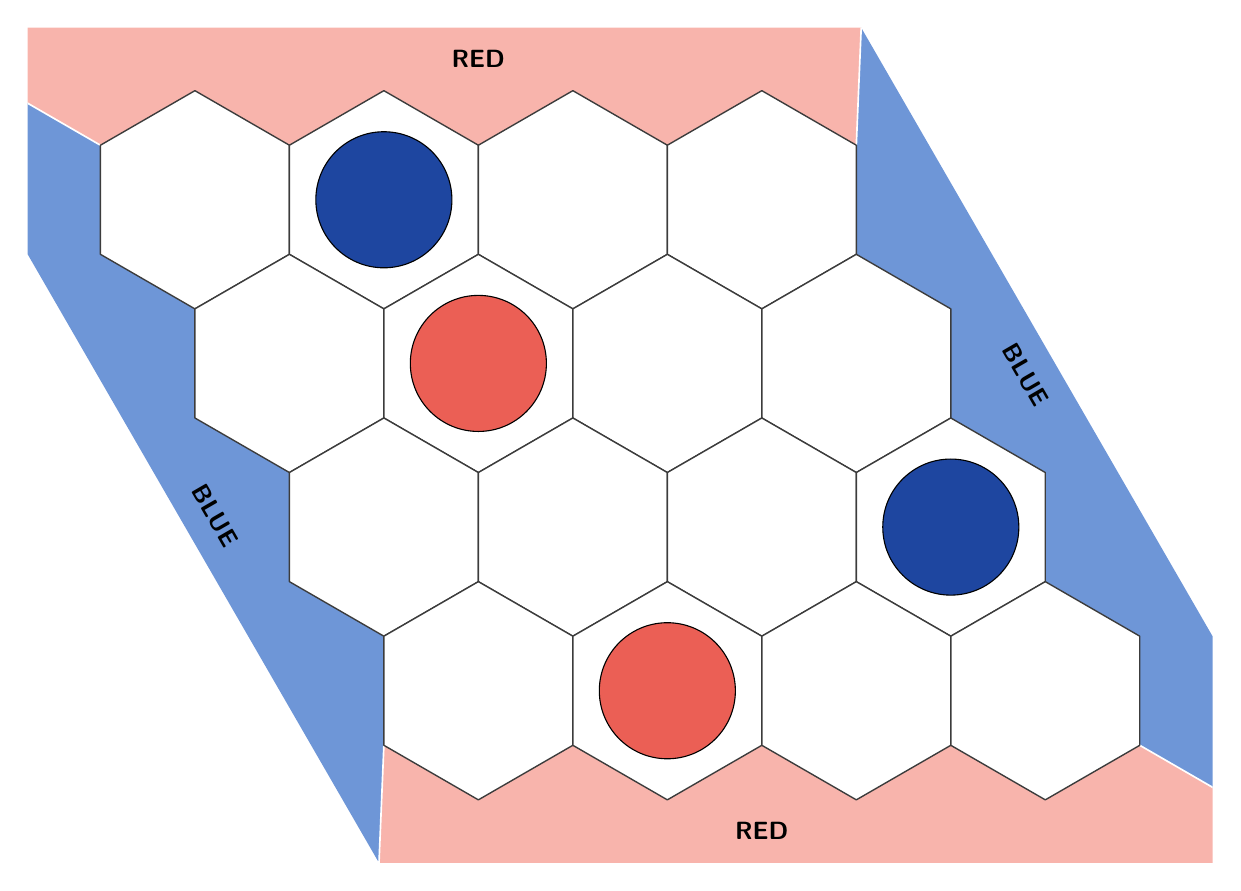
\begin{tikzpicture}[x=1.0mm,y=1.0mm,line join=round]
\begin{scope}
\clip (-21.238,-84.210) rectangle (129.238,21.856);
\fill[redtint] (-12.000,6.928) -- (0.000,13.856) -- (12.000,6.928) -- (24.000,13.856) -- (36.000,6.928) -- (48.000,13.856) -- (60.000,6.928) -- (72.000,13.856) -- (84.000,6.928) -- (84.619,21.856) -- (-37.856,21.856) -- cycle;
\fill[redtint] (120.000,-69.282) -- (108.000,-76.210) -- (96.000,-69.282) -- (84.000,-76.210) -- (72.000,-69.282) -- (60.000,-76.210) -- (48.000,-69.282) -- (36.000,-76.210) -- (24.000,-69.282) -- (23.381,-84.210) -- (145.856,-84.210) -- cycle;
\fill[bluetint] (24.000,-69.282) -- (24.000,-55.426) -- (12.000,-48.497) -- (12.000,-34.641) -- (0.000,-27.713) -- (-0.000,-13.856) -- (-12.000,-6.928) -- (-12.000,6.928) -- (-37.856,21.856) -- (23.381,-84.210) -- cycle;
\fill[bluetint] (84.000,6.928) -- (84.000,-6.928) -- (96.000,-13.856) -- (96.000,-27.713) -- (108.000,-34.641) -- (108.000,-48.497) -- (120.000,-55.426) -- (120.000,-69.282) -- (145.856,-84.210) -- (84.619,21.856) -- cycle;
\draw[white,line width=0.6pt] (-12.000,6.928) -- (-37.856,21.856);
\draw[white,line width=0.6pt] (84.000,6.928) -- (84.619,21.856);
\draw[white,line width=0.6pt] (120.000,-69.282) -- (145.856,-84.210);
\draw[white,line width=0.6pt] (24.000,-69.282) -- (23.381,-84.210);
\end{scope}
\node[font=\small\bfseries,text=black] at (36.000,17.856) {RED};
\node[font=\small\bfseries,text=black] at (72.000,-80.210) {RED};
\node[font=\small\bfseries,text=black,rotate=-60] at (2.536,-40.105) {BLUE};
\node[font=\small\bfseries,text=black,rotate=-60] at (105.464,-22.249) {BLUE};
\filldraw[fill=white,draw=gridline,line width=0.5pt] (12.000,6.928) -- (0.000,13.856) -- (-12.000,6.928) -- (-12.000,-6.928) -- (-0.000,-13.856) -- (12.000,-6.928) -- cycle;
\filldraw[fill=white,draw=gridline,line width=0.5pt] (36.000,6.928) -- (24.000,13.856) -- (12.000,6.928) -- (12.000,-6.928) -- (24.000,-13.856) -- (36.000,-6.928) -- cycle;
\filldraw[fill=white,draw=gridline,line width=0.5pt] (60.000,6.928) -- (48.000,13.856) -- (36.000,6.928) -- (36.000,-6.928) -- (48.000,-13.856) -- (60.000,-6.928) -- cycle;
\filldraw[fill=white,draw=gridline,line width=0.5pt] (84.000,6.928) -- (72.000,13.856) -- (60.000,6.928) -- (60.000,-6.928) -- (72.000,-13.856) -- (84.000,-6.928) -- cycle;
\filldraw[fill=white,draw=gridline,line width=0.5pt] (24.000,-13.856) -- (12.000,-6.928) -- (-0.000,-13.856) -- (0.000,-27.713) -- (12.000,-34.641) -- (24.000,-27.713) -- cycle;
\filldraw[fill=white,draw=gridline,line width=0.5pt] (48.000,-13.856) -- (36.000,-6.928) -- (24.000,-13.856) -- (24.000,-27.713) -- (36.000,-34.641) -- (48.000,-27.713) -- cycle;
\filldraw[fill=white,draw=gridline,line width=0.5pt] (72.000,-13.856) -- (60.000,-6.928) -- (48.000,-13.856) -- (48.000,-27.713) -- (60.000,-34.641) -- (72.000,-27.713) -- cycle;
\filldraw[fill=white,draw=gridline,line width=0.5pt] (96.000,-13.856) -- (84.000,-6.928) -- (72.000,-13.856) -- (72.000,-27.713) -- (84.000,-34.641) -- (96.000,-27.713) -- cycle;
\filldraw[fill=white,draw=gridline,line width=0.5pt] (36.000,-34.641) -- (24.000,-27.713) -- (12.000,-34.641) -- (12.000,-48.497) -- (24.000,-55.426) -- (36.000,-48.497) -- cycle;
\filldraw[fill=white,draw=gridline,line width=0.5pt] (60.000,-34.641) -- (48.000,-27.713) -- (36.000,-34.641) -- (36.000,-48.497) -- (48.000,-55.426) -- (60.000,-48.497) -- cycle;
\filldraw[fill=white,draw=gridline,line width=0.5pt] (84.000,-34.641) -- (72.000,-27.713) -- (60.000,-34.641) -- (60.000,-48.497) -- (72.000,-55.426) -- (84.000,-48.497) -- cycle;
\filldraw[fill=white,draw=gridline,line width=0.5pt] (108.000,-34.641) -- (96.000,-27.713) -- (84.000,-34.641) -- (84.000,-48.497) -- (96.000,-55.426) -- (108.000,-48.497) -- cycle;
\filldraw[fill=white,draw=gridline,line width=0.5pt] (48.000,-55.426) -- (36.000,-48.497) -- (24.000,-55.426) -- (24.000,-69.282) -- (36.000,-76.210) -- (48.000,-69.282) -- cycle;
\filldraw[fill=white,draw=gridline,line width=0.5pt] (72.000,-55.426) -- (60.000,-48.497) -- (48.000,-55.426) -- (48.000,-69.282) -- (60.000,-76.210) -- (72.000,-69.282) -- cycle;
\filldraw[fill=white,draw=gridline,line width=0.5pt] (96.000,-55.426) -- (84.000,-48.497) -- (72.000,-55.426) -- (72.000,-69.282) -- (84.000,-76.210) -- (96.000,-69.282) -- cycle;
\filldraw[fill=white,draw=gridline,line width=0.5pt] (120.000,-55.426) -- (108.000,-48.497) -- (96.000,-55.426) -- (96.000,-69.282) -- (108.000,-76.210) -- (120.000,-69.282) -- cycle;
\filldraw[fill=redctr,draw=black,line width=0.4pt] (36.000,-20.785) circle (8.640);
\filldraw[fill=redctr,draw=black,line width=0.4pt] (60.000,-62.354) circle (8.640);
\filldraw[fill=bluectr,draw=black,line width=0.4pt] (24.000,0.000) circle (8.640);
\filldraw[fill=bluectr,draw=black,line width=0.4pt] (96.000,-41.569) circle (8.640);
\end{tikzpicture}
\end{center}
\par\vspace{11mm}\noindent\begin{tikzpicture}[x=1mm,y=1mm]
\draw[writeline,line width=0.5pt] (0,0.0) -- (189.5,0.0);
\draw[writeline,line width=0.5pt] (0,-10.0) -- (189.5,-10.0);
\draw[writeline,line width=0.5pt] (0,-20.0) -- (189.5,-20.0);
\draw[writeline,line width=0.5pt] (0,-30.0) -- (189.5,-30.0);
\draw[writeline,line width=0.5pt] (0,-40.0) -- (189.5,-40.0);
\end{tikzpicture}\par

\clearpage
\prob{10} Hex players often use a board with 11 rows of 11 hexagons. Nobody knows a sure way to win on it. Maya says she has a way to always win on that board when she goes second, playing by the rules on page 1. Explain why Maya must be wrong.\par\vspace{11mm}\noindent\begin{tikzpicture}[x=1mm,y=1mm]
\draw[writeline,line width=0.5pt] (0,0.0) -- (189.5,0.0);
\draw[writeline,line width=0.5pt] (0,-10.0) -- (189.5,-10.0);
\draw[writeline,line width=0.5pt] (0,-20.0) -- (189.5,-20.0);
\draw[writeline,line width=0.5pt] (0,-30.0) -- (189.5,-30.0);
\draw[writeline,line width=0.5pt] (0,-40.0) -- (189.5,-40.0);
\draw[writeline,line width=0.5pt] (0,-50.0) -- (189.5,-50.0);
\draw[writeline,line width=0.5pt] (0,-60.0) -- (189.5,-60.0);
\draw[writeline,line width=0.5pt] (0,-70.0) -- (189.5,-70.0);
\draw[writeline,line width=0.5pt] (0,-80.0) -- (189.5,-80.0);
\draw[writeline,line width=0.5pt] (0,-90.0) -- (189.5,-90.0);
\draw[writeline,line width=0.5pt] (0,-100.0) -- (189.5,-100.0);
\draw[writeline,line width=0.5pt] (0,-110.0) -- (189.5,-110.0);
\draw[writeline,line width=0.5pt] (0,-120.0) -- (189.5,-120.0);
\draw[writeline,line width=0.5pt] (0,-130.0) -- (189.5,-130.0);
\end{tikzpicture}\par

\clearpage
\sbox{\landbox}{\begin{minipage}{254mm}\large\prob{11} Play Hex on this board. Take turns going first.\par\vspace{3mm}\centering 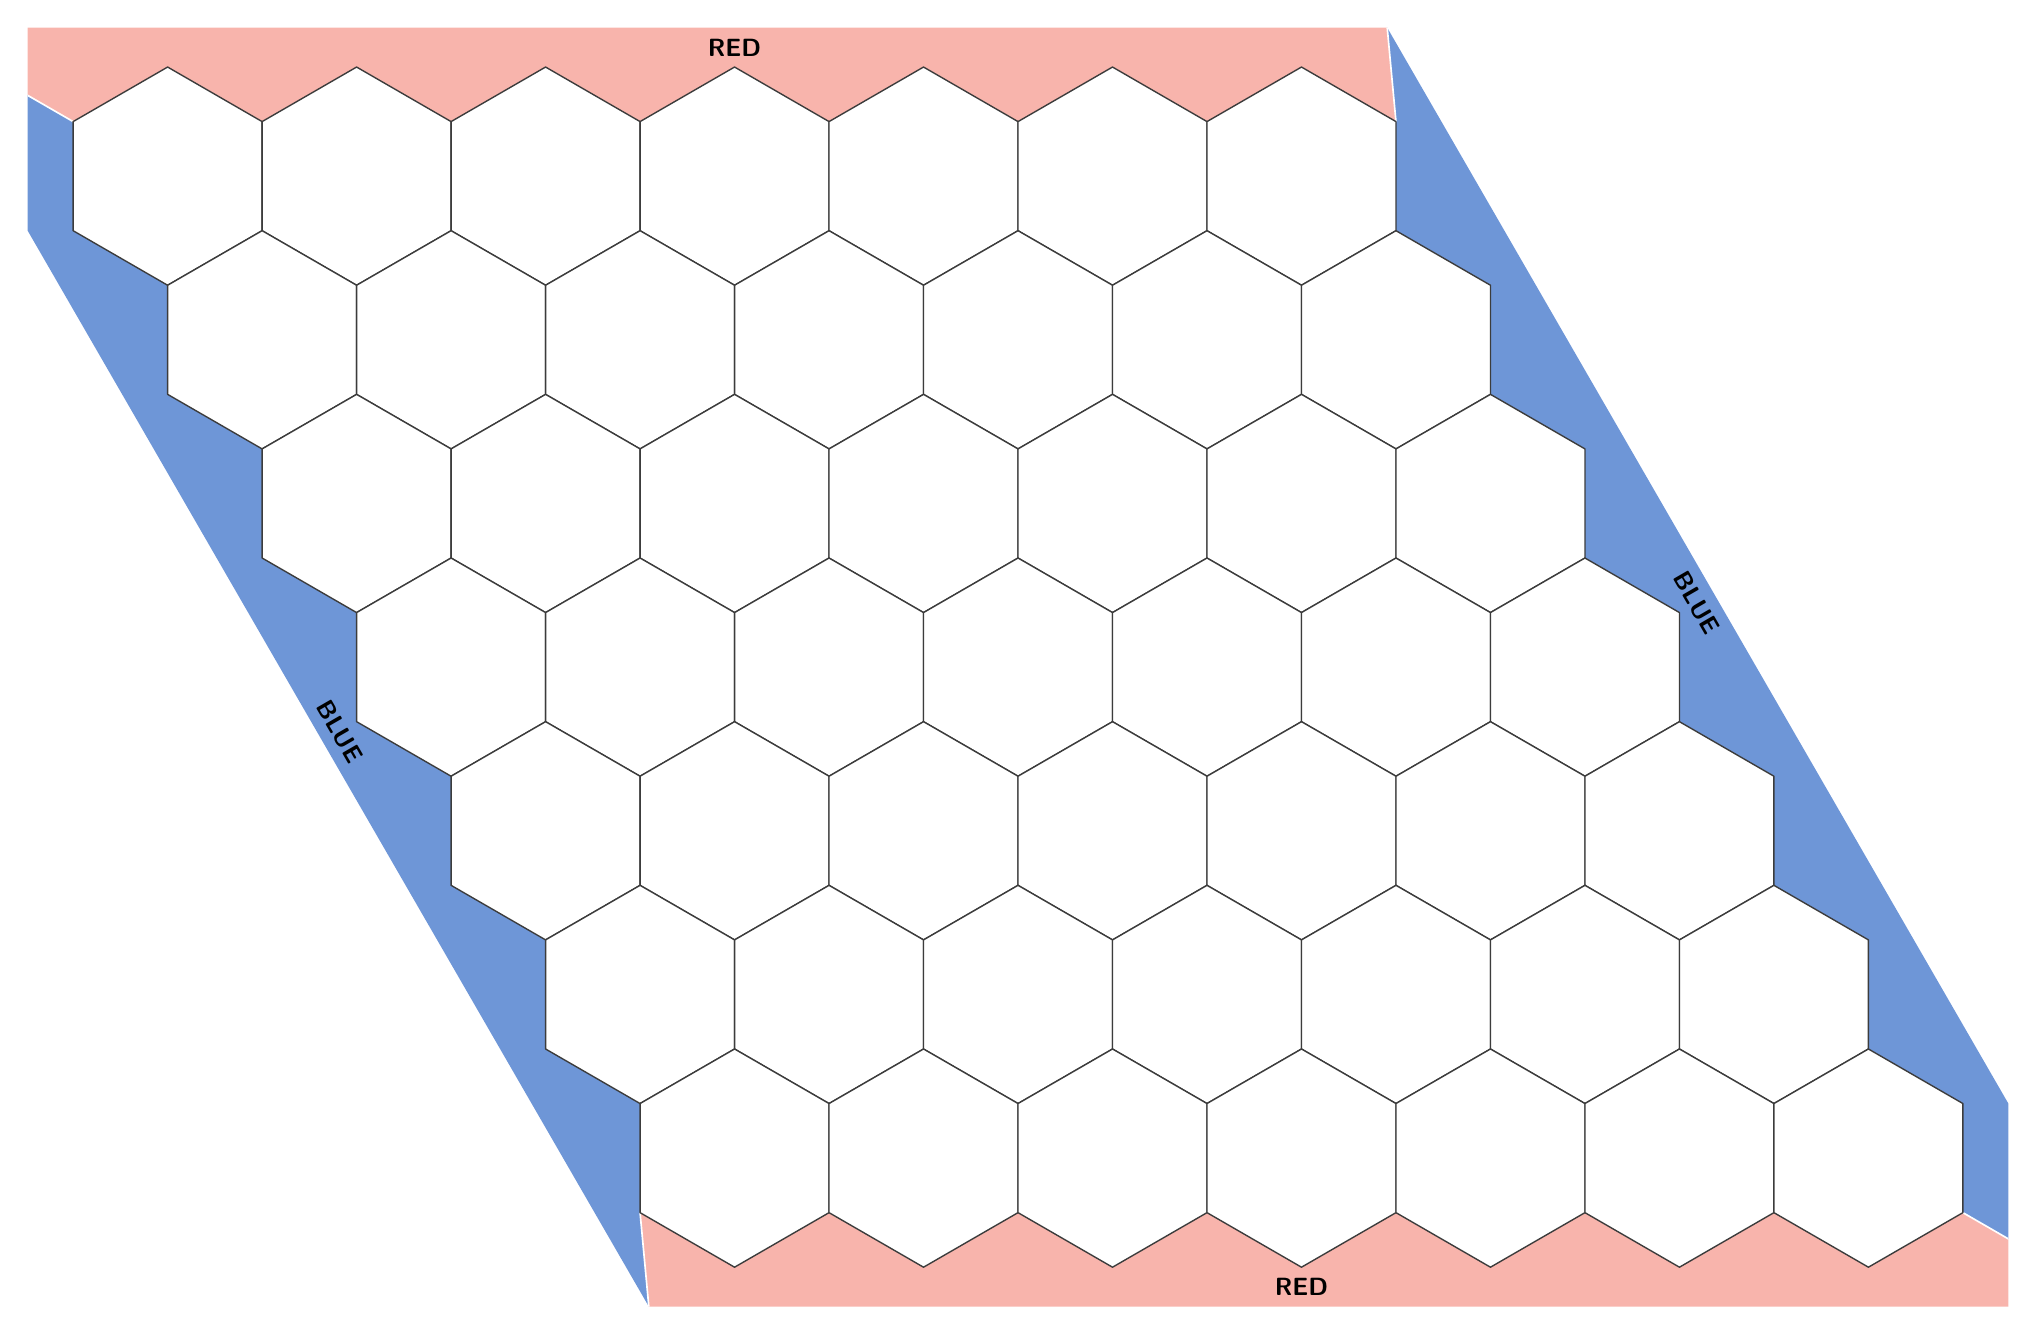
\begin{tikzpicture}[x=1.0mm,y=1.0mm,line join=round]
\begin{scope}
\clip (-17.774,-143.564) rectangle (233.774,18.856);
\fill[redtint] (-12.000,6.928) -- (0.000,13.856) -- (12.000,6.928) -- (24.000,13.856) -- (36.000,6.928) -- (48.000,13.856) -- (60.000,6.928) -- (72.000,13.856) -- (84.000,6.928) -- (96.000,13.856) -- (108.000,6.928) -- (120.000,13.856) -- (132.000,6.928) -- (144.000,13.856) -- (156.000,6.928) -- (154.887,18.856) -- (-32.660,18.856) -- cycle;
\fill[redtint] (228.000,-131.636) -- (216.000,-138.564) -- (204.000,-131.636) -- (192.000,-138.564) -- (180.000,-131.636) -- (168.000,-138.564) -- (156.000,-131.636) -- (144.000,-138.564) -- (132.000,-131.636) -- (120.000,-138.564) -- (108.000,-131.636) -- (96.000,-138.564) -- (84.000,-131.636) -- (72.000,-138.564) -- (60.000,-131.636) -- (61.113,-143.564) -- (248.660,-143.564) -- cycle;
\fill[bluetint] (60.000,-131.636) -- (60.000,-117.779) -- (48.000,-110.851) -- (48.000,-96.995) -- (36.000,-90.067) -- (36.000,-76.210) -- (24.000,-69.282) -- (24.000,-55.426) -- (12.000,-48.497) -- (12.000,-34.641) -- (0.000,-27.713) -- (-0.000,-13.856) -- (-12.000,-6.928) -- (-12.000,6.928) -- (-32.660,18.856) -- (61.113,-143.564) -- cycle;
\fill[bluetint] (156.000,6.928) -- (156.000,-6.928) -- (168.000,-13.856) -- (168.000,-27.713) -- (180.000,-34.641) -- (180.000,-48.497) -- (192.000,-55.426) -- (192.000,-69.282) -- (204.000,-76.210) -- (204.000,-90.067) -- (216.000,-96.995) -- (216.000,-110.851) -- (228.000,-117.779) -- (228.000,-131.636) -- (248.660,-143.564) -- (154.887,18.856) -- cycle;
\draw[white,line width=0.6pt] (-12.000,6.928) -- (-32.660,18.856);
\draw[white,line width=0.6pt] (156.000,6.928) -- (154.887,18.856);
\draw[white,line width=0.6pt] (228.000,-131.636) -- (248.660,-143.564);
\draw[white,line width=0.6pt] (60.000,-131.636) -- (61.113,-143.564);
\end{scope}
\node[font=\small\bfseries,text=black] at (72.000,16.356) {RED};
\node[font=\small\bfseries,text=black] at (144.000,-141.064) {RED};
\node[font=\small\bfseries,text=black,rotate=-60] at (21.835,-70.532) {BLUE};
\node[font=\small\bfseries,text=black,rotate=-60] at (194.165,-54.176) {BLUE};
\filldraw[fill=white,draw=gridline,line width=0.5pt] (12.000,6.928) -- (0.000,13.856) -- (-12.000,6.928) -- (-12.000,-6.928) -- (-0.000,-13.856) -- (12.000,-6.928) -- cycle;
\filldraw[fill=white,draw=gridline,line width=0.5pt] (36.000,6.928) -- (24.000,13.856) -- (12.000,6.928) -- (12.000,-6.928) -- (24.000,-13.856) -- (36.000,-6.928) -- cycle;
\filldraw[fill=white,draw=gridline,line width=0.5pt] (60.000,6.928) -- (48.000,13.856) -- (36.000,6.928) -- (36.000,-6.928) -- (48.000,-13.856) -- (60.000,-6.928) -- cycle;
\filldraw[fill=white,draw=gridline,line width=0.5pt] (84.000,6.928) -- (72.000,13.856) -- (60.000,6.928) -- (60.000,-6.928) -- (72.000,-13.856) -- (84.000,-6.928) -- cycle;
\filldraw[fill=white,draw=gridline,line width=0.5pt] (108.000,6.928) -- (96.000,13.856) -- (84.000,6.928) -- (84.000,-6.928) -- (96.000,-13.856) -- (108.000,-6.928) -- cycle;
\filldraw[fill=white,draw=gridline,line width=0.5pt] (132.000,6.928) -- (120.000,13.856) -- (108.000,6.928) -- (108.000,-6.928) -- (120.000,-13.856) -- (132.000,-6.928) -- cycle;
\filldraw[fill=white,draw=gridline,line width=0.5pt] (156.000,6.928) -- (144.000,13.856) -- (132.000,6.928) -- (132.000,-6.928) -- (144.000,-13.856) -- (156.000,-6.928) -- cycle;
\filldraw[fill=white,draw=gridline,line width=0.5pt] (24.000,-13.856) -- (12.000,-6.928) -- (-0.000,-13.856) -- (0.000,-27.713) -- (12.000,-34.641) -- (24.000,-27.713) -- cycle;
\filldraw[fill=white,draw=gridline,line width=0.5pt] (48.000,-13.856) -- (36.000,-6.928) -- (24.000,-13.856) -- (24.000,-27.713) -- (36.000,-34.641) -- (48.000,-27.713) -- cycle;
\filldraw[fill=white,draw=gridline,line width=0.5pt] (72.000,-13.856) -- (60.000,-6.928) -- (48.000,-13.856) -- (48.000,-27.713) -- (60.000,-34.641) -- (72.000,-27.713) -- cycle;
\filldraw[fill=white,draw=gridline,line width=0.5pt] (96.000,-13.856) -- (84.000,-6.928) -- (72.000,-13.856) -- (72.000,-27.713) -- (84.000,-34.641) -- (96.000,-27.713) -- cycle;
\filldraw[fill=white,draw=gridline,line width=0.5pt] (120.000,-13.856) -- (108.000,-6.928) -- (96.000,-13.856) -- (96.000,-27.713) -- (108.000,-34.641) -- (120.000,-27.713) -- cycle;
\filldraw[fill=white,draw=gridline,line width=0.5pt] (144.000,-13.856) -- (132.000,-6.928) -- (120.000,-13.856) -- (120.000,-27.713) -- (132.000,-34.641) -- (144.000,-27.713) -- cycle;
\filldraw[fill=white,draw=gridline,line width=0.5pt] (168.000,-13.856) -- (156.000,-6.928) -- (144.000,-13.856) -- (144.000,-27.713) -- (156.000,-34.641) -- (168.000,-27.713) -- cycle;
\filldraw[fill=white,draw=gridline,line width=0.5pt] (36.000,-34.641) -- (24.000,-27.713) -- (12.000,-34.641) -- (12.000,-48.497) -- (24.000,-55.426) -- (36.000,-48.497) -- cycle;
\filldraw[fill=white,draw=gridline,line width=0.5pt] (60.000,-34.641) -- (48.000,-27.713) -- (36.000,-34.641) -- (36.000,-48.497) -- (48.000,-55.426) -- (60.000,-48.497) -- cycle;
\filldraw[fill=white,draw=gridline,line width=0.5pt] (84.000,-34.641) -- (72.000,-27.713) -- (60.000,-34.641) -- (60.000,-48.497) -- (72.000,-55.426) -- (84.000,-48.497) -- cycle;
\filldraw[fill=white,draw=gridline,line width=0.5pt] (108.000,-34.641) -- (96.000,-27.713) -- (84.000,-34.641) -- (84.000,-48.497) -- (96.000,-55.426) -- (108.000,-48.497) -- cycle;
\filldraw[fill=white,draw=gridline,line width=0.5pt] (132.000,-34.641) -- (120.000,-27.713) -- (108.000,-34.641) -- (108.000,-48.497) -- (120.000,-55.426) -- (132.000,-48.497) -- cycle;
\filldraw[fill=white,draw=gridline,line width=0.5pt] (156.000,-34.641) -- (144.000,-27.713) -- (132.000,-34.641) -- (132.000,-48.497) -- (144.000,-55.426) -- (156.000,-48.497) -- cycle;
\filldraw[fill=white,draw=gridline,line width=0.5pt] (180.000,-34.641) -- (168.000,-27.713) -- (156.000,-34.641) -- (156.000,-48.497) -- (168.000,-55.426) -- (180.000,-48.497) -- cycle;
\filldraw[fill=white,draw=gridline,line width=0.5pt] (48.000,-55.426) -- (36.000,-48.497) -- (24.000,-55.426) -- (24.000,-69.282) -- (36.000,-76.210) -- (48.000,-69.282) -- cycle;
\filldraw[fill=white,draw=gridline,line width=0.5pt] (72.000,-55.426) -- (60.000,-48.497) -- (48.000,-55.426) -- (48.000,-69.282) -- (60.000,-76.210) -- (72.000,-69.282) -- cycle;
\filldraw[fill=white,draw=gridline,line width=0.5pt] (96.000,-55.426) -- (84.000,-48.497) -- (72.000,-55.426) -- (72.000,-69.282) -- (84.000,-76.210) -- (96.000,-69.282) -- cycle;
\filldraw[fill=white,draw=gridline,line width=0.5pt] (120.000,-55.426) -- (108.000,-48.497) -- (96.000,-55.426) -- (96.000,-69.282) -- (108.000,-76.210) -- (120.000,-69.282) -- cycle;
\filldraw[fill=white,draw=gridline,line width=0.5pt] (144.000,-55.426) -- (132.000,-48.497) -- (120.000,-55.426) -- (120.000,-69.282) -- (132.000,-76.210) -- (144.000,-69.282) -- cycle;
\filldraw[fill=white,draw=gridline,line width=0.5pt] (168.000,-55.426) -- (156.000,-48.497) -- (144.000,-55.426) -- (144.000,-69.282) -- (156.000,-76.210) -- (168.000,-69.282) -- cycle;
\filldraw[fill=white,draw=gridline,line width=0.5pt] (192.000,-55.426) -- (180.000,-48.497) -- (168.000,-55.426) -- (168.000,-69.282) -- (180.000,-76.210) -- (192.000,-69.282) -- cycle;
\filldraw[fill=white,draw=gridline,line width=0.5pt] (60.000,-76.210) -- (48.000,-69.282) -- (36.000,-76.210) -- (36.000,-90.067) -- (48.000,-96.995) -- (60.000,-90.067) -- cycle;
\filldraw[fill=white,draw=gridline,line width=0.5pt] (84.000,-76.210) -- (72.000,-69.282) -- (60.000,-76.210) -- (60.000,-90.067) -- (72.000,-96.995) -- (84.000,-90.067) -- cycle;
\filldraw[fill=white,draw=gridline,line width=0.5pt] (108.000,-76.210) -- (96.000,-69.282) -- (84.000,-76.210) -- (84.000,-90.067) -- (96.000,-96.995) -- (108.000,-90.067) -- cycle;
\filldraw[fill=white,draw=gridline,line width=0.5pt] (132.000,-76.210) -- (120.000,-69.282) -- (108.000,-76.210) -- (108.000,-90.067) -- (120.000,-96.995) -- (132.000,-90.067) -- cycle;
\filldraw[fill=white,draw=gridline,line width=0.5pt] (156.000,-76.210) -- (144.000,-69.282) -- (132.000,-76.210) -- (132.000,-90.067) -- (144.000,-96.995) -- (156.000,-90.067) -- cycle;
\filldraw[fill=white,draw=gridline,line width=0.5pt] (180.000,-76.210) -- (168.000,-69.282) -- (156.000,-76.210) -- (156.000,-90.067) -- (168.000,-96.995) -- (180.000,-90.067) -- cycle;
\filldraw[fill=white,draw=gridline,line width=0.5pt] (204.000,-76.210) -- (192.000,-69.282) -- (180.000,-76.210) -- (180.000,-90.067) -- (192.000,-96.995) -- (204.000,-90.067) -- cycle;
\filldraw[fill=white,draw=gridline,line width=0.5pt] (72.000,-96.995) -- (60.000,-90.067) -- (48.000,-96.995) -- (48.000,-110.851) -- (60.000,-117.779) -- (72.000,-110.851) -- cycle;
\filldraw[fill=white,draw=gridline,line width=0.5pt] (96.000,-96.995) -- (84.000,-90.067) -- (72.000,-96.995) -- (72.000,-110.851) -- (84.000,-117.779) -- (96.000,-110.851) -- cycle;
\filldraw[fill=white,draw=gridline,line width=0.5pt] (120.000,-96.995) -- (108.000,-90.067) -- (96.000,-96.995) -- (96.000,-110.851) -- (108.000,-117.779) -- (120.000,-110.851) -- cycle;
\filldraw[fill=white,draw=gridline,line width=0.5pt] (144.000,-96.995) -- (132.000,-90.067) -- (120.000,-96.995) -- (120.000,-110.851) -- (132.000,-117.779) -- (144.000,-110.851) -- cycle;
\filldraw[fill=white,draw=gridline,line width=0.5pt] (168.000,-96.995) -- (156.000,-90.067) -- (144.000,-96.995) -- (144.000,-110.851) -- (156.000,-117.779) -- (168.000,-110.851) -- cycle;
\filldraw[fill=white,draw=gridline,line width=0.5pt] (192.000,-96.995) -- (180.000,-90.067) -- (168.000,-96.995) -- (168.000,-110.851) -- (180.000,-117.779) -- (192.000,-110.851) -- cycle;
\filldraw[fill=white,draw=gridline,line width=0.5pt] (216.000,-96.995) -- (204.000,-90.067) -- (192.000,-96.995) -- (192.000,-110.851) -- (204.000,-117.779) -- (216.000,-110.851) -- cycle;
\filldraw[fill=white,draw=gridline,line width=0.5pt] (84.000,-117.779) -- (72.000,-110.851) -- (60.000,-117.779) -- (60.000,-131.636) -- (72.000,-138.564) -- (84.000,-131.636) -- cycle;
\filldraw[fill=white,draw=gridline,line width=0.5pt] (108.000,-117.779) -- (96.000,-110.851) -- (84.000,-117.779) -- (84.000,-131.636) -- (96.000,-138.564) -- (108.000,-131.636) -- cycle;
\filldraw[fill=white,draw=gridline,line width=0.5pt] (132.000,-117.779) -- (120.000,-110.851) -- (108.000,-117.779) -- (108.000,-131.636) -- (120.000,-138.564) -- (132.000,-131.636) -- cycle;
\filldraw[fill=white,draw=gridline,line width=0.5pt] (156.000,-117.779) -- (144.000,-110.851) -- (132.000,-117.779) -- (132.000,-131.636) -- (144.000,-138.564) -- (156.000,-131.636) -- cycle;
\filldraw[fill=white,draw=gridline,line width=0.5pt] (180.000,-117.779) -- (168.000,-110.851) -- (156.000,-117.779) -- (156.000,-131.636) -- (168.000,-138.564) -- (180.000,-131.636) -- cycle;
\filldraw[fill=white,draw=gridline,line width=0.5pt] (204.000,-117.779) -- (192.000,-110.851) -- (180.000,-117.779) -- (180.000,-131.636) -- (192.000,-138.564) -- (204.000,-131.636) -- cycle;
\filldraw[fill=white,draw=gridline,line width=0.5pt] (228.000,-117.779) -- (216.000,-110.851) -- (204.000,-117.779) -- (204.000,-131.636) -- (216.000,-138.564) -- (228.000,-131.636) -- cycle;
\end{tikzpicture}\end{minipage}}
\pdfpageattr{/Rotate 90}
\thispagestyle{empty}
\begin{tikzpicture}[remember picture,overlay]
\begin{scope}[shift={(current page.center)},rotate=90,transform shape]
\node[anchor=base west,inner sep=0pt] at (-127mm,94mm) {Week NN / Hex / Grades 4--5};
\node[anchor=base west,inner sep=0pt] at (-127mm,-97.8mm) {Bellingham Math Circle / Week NN / HEX-45-v1};
\node[anchor=base east,inner sep=0pt] at (127mm,-97.8mm) {\thepage};
\node[anchor=north,inner sep=0pt] at (0,87mm) {\usebox{\landbox}};
\end{scope}
\end{tikzpicture}
\mbox{}
\clearpage
\pdfpageattr{}

\end{document}
